\chapter{Dinámica neuronal en el conectoma del C. elegans}\label{cap:resultado_critico_modelo}
\graphicspath{{figs/capitulo_resultado_critico/}}

\chapterquote{My question is, \textquote{can physics be simulated by a universal computer?}. . . I would like to have the elements of this computer locally 	interconnected, and therefore sort of think about cellular automata as an example. . . We might change the idea that space is continuous to the 	idea that space perhaps is a simple lattice and everything is discrete. . .and that time jumps discontinously. }{Richard P. Feynman}

En este apartado, se exponen los resultados derivados de nuestro modelo computacional basado en el conectoma del nematodo C. elegans. Nuestro enfoque en este capítulo consiste en explorar cómo emergen las propiedades de la criticidad neuronal en un sistema nervioso simplificado y modelado. Esta perspectiva nos permite analizar las dinámicas neuronales a nivel macroscópico y determinar si el C. elegans manifiesta propiedades de criticidad neuronal a nivel global.

A lo largo de este capítulo, se describirá minuciosamente el modelo computacional utilizado, incluyendo sus parámetros y suposiciones subyacentes. Se presentarán los resultados de las simulaciones y se examinará cómo la manipulación de los parámetros de la dinámica neuronal y del sistema en su conjunto influye en la emergencia de la criticidad neuronal.

De manera similar al capítulo anterior, se evaluará la coherencia de los hallazgos con la teoría de la criticidad neuronal y se explorará su relevancia en los campos de la neurociencia y la computación neuronal. Se discutirán las contribuciones específicas de nuestro modelo y cómo complementa los resultados obtenidos a partir de los datos experimentales. Además, se considerarán las posibles limitaciones y futuras direcciones de esta investigación interdisciplinaria.


\section{Modelo computacional de dinámica neuronal}




%Emergent Complexity is Always Critical
%
%La comunalidad de la dinámica libre de escala en el cerebro nos lleva naturalmente a preguntarnos qué sabe la física sobre mecanismos muy generales que son capaces de producir tal dinámica. Los intentos de explicar y generar la no uniformidad de la naturaleza incluyeron varios modelos y recetas matemáticos, pero pocos lograron crear complejidad sin incrustar las ecuaciones con complejidad. El punto importante es que incluir la complejidad en el modelo solo resultará en una simulación del sistema real, sin implicar ninguna comprensión de la complejidad. Los esfuerzos más significativos fueron aquellos destinados a descubrir las condiciones en las que algo complejo emerge de la interacción de los elementos constituyentes no complejos [1, 9].
%
%
%
%Los intentos de construir modelos de equilibrio biológicamente realistas de redes neuronales requieren como ingrediente principal la introducción de ruido (a veces finamente afinado) (Deco et al., 2009; Rolls y Deco, 2010). En este tipo de modelos, sin el ruido externo la dinámica se atasca en un estado de equilibrio estable, por lo que el ruido debe ser introducido ad hoc para permitir suficiente variabilidad en el comportamiento dinámico del sistema. Sin embargo, hay que ser muy cuidadoso para no sobreestimar la relevancia biológica de una construcción necesaria para superar las deficiencias de una clase restringida de modelos. Los resultados de la física estadística nos dicen que las fluctuaciones dinámicas en torno a los estados estacionarios son pequeñas, excepto cerca de los puntos críticos (Prigogine, 1962). Por el contrario, un sistema fuera de equilibrio que sufre criticidad no necesita la introducción de ruido: la variabilidad es autogenerada por la dinámica colectiva que fluctúa espontáneamente cerca del punto crítico (para una discusión más detallada, véase (Tagliazucchi y Chialvo, 2011)). Casualmente, los resultados actuales muestran que la organización espaciotemporal de la dinámica cerebral en reposo alcanza la máxima variabilidad (es )3C,E) a un nivel particular de activación, y el análisis de los parámetros de orden y control revela que el origen de dicha variabilidad puede, de hecho, rastrearse hasta una transición de fase. Además, el nivel de actividad pasa la mayor cantidad de tiempo alrededor de dicha transición. Por lo tanto, estos resultados apuntan a que se necesita una clase diferente de modelos: uno que enfatice la variabilidad autogenerada fuera de equilibrio sobre el ruido introducido ad hoc de origen incierto.
%
%
%
%
%%  Brain complexity born out of criticality Enzo Tagliazucchi ∗ and Dante R Chialvo†
%
%A pesar de lo convincentes que puedan ser los hallazgos experimentales de invariancia de escala anteriores, no revelan pistas sobre su origen. Eventualmente, lo que se necesita es identificar a partir de los datos los elementos fundamentales de una transición de fase de segundo orden, a saber, los cambios dinámicos en un parámetro de orden en función de algún parámetro de control. La derivación de estos no es necesaria solo por razones teóricas, sino que también tiene una importante relevancia práctica: un parámetro de control permite cuantificar el "grado de criticidad" presente en el sistema. Como en cualquier sistema finito fuera de equilibrio, las fluctuaciones de la actividad cerebral imponen cambios espontáneos en el régimen dinámico. Un parámetro de orden y control permitiría, por ejemplo, disipar la idea de que el régimen dinámico del cerebro es fijo y, por lo tanto, estudiar el impacto de la criticidad en los aspectos fluctuantes espontáneos del comportamiento y la cognición.
%
%El parámetro de control definido aquí es aproximadamente equivalente al nivel de actividad global instantáneo. El parámetro de orden es equivalente al tamaño del grupo más grande de actividad cortical activada (normalizado por el nivel de actividad global). Con estas definiciones, un diagrama de dispersión de orden frente a parámetros de control mostró una transición brusca alrededor de un nivel crítico de actividad global, produciendo un diagrama que se asemeja a los derivados para otros sistemas que experimentan una transición de fase de segundo orden.




Algunos aspectos cruciales de la dinámica neuronal  de los experimentos discutidos en la apartado anterior se reproducen bien en el régimen crítico del modelo de autómata celular desarrollado en el  \cref{titulo-modelo-criticidad}. En este apartado, demostramos las características cuantitativas del modelo computacional y discutimos su relación con estados críticos y no críticos.  Para simular la actividad neuronal a nivel de todo el cerebro, empleamos el modelo de dinámicas estocásticas basado en un autómata celular discreto desarrollado por Haimovici et al.   La \Cref{fig:spikeautomata} ilustra los principales ingredientes de nuestra estrategia de modelado.  La  matriz de adjacencia del conectoma del C. elegans es  la entrada clave del modelo estocástico (\Cref{fig:spikeautomata} Derecha).  El sistema se describe como un grafo  de $N$  nodos que se corresponde con las neuronas del C. elegans.  El grafo del conectoma hermafrodita tiene  $302$ nodos, mientras que el grafo del macho tiene $385$ nodos.  Los pesos de la matriz de adyacencia, $W_{i j}$  indican la cantidad total de conectividad física entre cada par de neuronas.  Los grafos respectivos tienen $4887$ enlaces químicos (o dirigidos)  en el hermafrodita y $5315$ enlaces químicos  en el macho. Son grafos dispersos con respectivamente 3,2\% (para el hermafrodita) y 2,4\% (para el macho) de todos los enlaces posibles.   Aunque es escaso, si se considera que todos los enlaces para ambos sexos no están dirigidos existe  una ruta que conecta cada par de nodos (débilmente conectados).  La figura 1A muestra la topografía de las conexiones estructurales, la asignación de red correspondiente y la matriz estructural correspondiente.


La dinámica del modelo es discreta. En cada paso, una neurona está en uno de los tres estados: quiescente ($Q$), excitado ($E$), o refractario ($R$). Una configuración global $\mathbf{s} \in \varepsilon^N$ del autómata está determinada por los valores de estado de todas las $N$ neuronas en la red (fig. 4.10), es decir, $\mathbf{s} \coloneq \left(s_1,\cdots,s_N  \right)=\left(s_i\right)_{i\in N}$.  Este vector asume valores en el espacio de estado $\mathcal{S} = \mathcal{E}^N$.  El estado de una neurona $i$, $s_i(t)$, se establece en $1$ si la neurona está activa, $0.5$ si esta refractario  y $0$  si se encuentra  en el estado quiescente. La dinámica temporal de la $i$-ésima neurona se rige por las probabilidades de transición entre un par de estados que fueron presantadas en  la   \cref{def_modelo}.  La \Cref{fig:modelopasos}  muestra un ejemplo ilustrativo de estas transiciones.  El estado de cada neurona se sobrescribe sólo después de que se actualice toda la red es decir el autómata celular tendrá una actualización sincrónica. Por lo tanto, durante la dinámica temporal, la activación de un nodo ocurre (más frecuentemente) cuando la excitación de entrada entrante de sus vecinos activos más cercanos excede un umbral fijo $T$, es decir, $\sum_j W_{ji}\delta_{j,1}>T$. En otras palabras, $T$ juega el papel de un parámetro de umbral que regula la propagación de la actividad excitatoria entrante.

Denotamos la configuración global en pasos de tiempo discretos posteriores $t \in \mathbb{N}_0$ como $\mathbf{s}(t) = (s_1(t),\cdots , s_N(t))\in \mathcal{S}$, donde $s_i(t) \in \mathcal{E}$ es el estado de la neurona $i$ en el tiempo $t$.  Para cada configuración global inicial  $\mathbf{s} (t=0) \in \mathcal{S}$, el desarrollo temporal del sistema está determinado por $\mathbf{s}(t+1)=\mathcal{R}_g(\mathbf{s}(t))$, donde la dinámica de un estado $s_i$ se determina mediante $s_i(t+1)=\mathcal{R}\left(\mathbf{s}_{\mathcal{N}(i)}(t)\right)$.


\begin{figure}[h!]
	\centering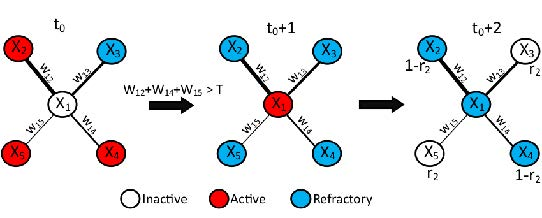
\includegraphics[width=\imsize]{modelopasos}
	\caption[Ejemplo de transiciones dinámicas en el modelo.]{Ejemplo de transiciones dinámicas en el modelo: en $t = t_0$ las neuronas activas son $x_2$,$x_4$ y $x_5$, que excitan $x_1$ en $t = t_0 + 1$, y luego ingresan al estado refractario con $t = t_0 + 2$, $x_3$ y $x_5$ se han recuperado y son susceptibles de excitarse nuevamente,
		mientras que $x_2$ y $x_4$ siguen siendo refractarios.} \label{fig:modelopasos}
\end{figure}





\subsection{Caracterización de la dinámica neuronal simulada}

Todas las simulaciones computacionales de este capitulo se realizaron en Python 3. Con el fin de obtener buenas estadísticas para las funciones de distribución de probabilidad, los parámetros de orden así como otras firmas de criticidad,  realizamos simulaciones para $100$ realizaciones diferentes del modelo  y $5000$ pasos de tiempo para cada realización. En la simulación numérica se ha discretizado el tiempo en pasos $dt$.  Para cada valor del umbral $T$  se calculan las variables macroscópicas que caracterizan al sistema,  el calculo se realiza simulando distintas configuraciones del sistema  donde para cada una de estas  los estados iniciales de la red son  tomados de forma aleatoria del vector de estados.     Los promedios sobre configuraciones se calculan  mediante

\begin{equation}\label{eq:63}
	\left\langle X\right\rangle_c \coloneqq  \frac{1}{M}\sum_{i=1}^{M} \left\langle X \right\rangle_t 
\end{equation}

donde $\left\langle X \right\rangle_t $  es el promedio temporal de la variable $X$ y $\left\langle X\right\rangle_c$ es el promedio sobre un total de $M$ configuraciones del sistema. A lo largo de este capitulo, a menos que se indique lo contrario, los resultados numéricos finales presentados fueron promedios de $100$ configuraciones  con condiciones iniciales aleatorias, para un total de $t_s$ pasos de tiempo.  En cada una de estas configuraciones para cada punto de tiempo  exploramos un conjunto de diferentes métricas para describir la dinámica del modelo. Su elección estuvo motivada por que  se ha demostrado previamente que se comportan de manera diferente en los casos supercrítico, subcrítico y crítico (ya sea teórica o empíricamente). Se investigaron las siguientes métricas:



\begin{itemize}
	\item  la actividad media de la red,
	\begin{equation}\label{eq:58}
		\left\langle A(t)\right\rangle_t  = \bar{A(t)} = \frac{1}{t_s-\tau_1}\sum_{t=\tau_1}^{t_s} A(t),
	\end{equation}
	donde 
	\begin{equation}\label{eq:59}
		A(t) = \frac{1}{N}\sum_{i=1}^{N} \delta_{s_i(t),E}
	\end{equation}
	corresponde a la fracción de neuronas activas en el tiempo $t$, es decir  es la actividad instantánea, $N$ es el número total de neuronas, $\tau_1$ es el tiempo de relajación, esto es el tiempo característico que demora el sistema en alcanzar un estado estacionario a partir de un estado inicial aleatorio arbitrario y $t_s$ es el tiempo total de simulación;
	\item la desviación estándar de $A(t)$,
	
	\begin{equation}
		\sigma_A=\sqrt{\frac{1}{t_s-\tau_1}\sum_{t=\tau_1}^{t_s}\left(A(t)-\left\langle  A\right\rangle \right)^2}
	\end{equation}
	Estas métricas capturan el grado de actividad y si la dinámica cerebral global presenta variabilidad temporal o es relativamente constante en el tiempo.
	\item el tamaño del promedio de los clústeres $\chi$, el primer clúster más grande $\bar{S}_1$ y  el tamaño del segundo clúster más grande ($\bar{S}_2$) los cuales fueron definidos en el \Cref{sec:percolacion_critico}. $\bar{S}_2$  en contraste con  $\bar{S}_1$ (que crece monótonamente a medida que aumenta la actividad en el modelo), $\bar{S}_2$ alcanza su punto máximo justo antes de que la actividad se fusione en un componente conectado gigante y luego disminuye. Estas dos métricas son parámetros de orden estándar en la teoría de la percolación \cite{stauffer_scaling_1979} y también se han empleado como parámetros de orden para el modelo de GreenbergHastings \cite{haimovici_brain_2013}. Biológicamente, $\bar{S}_2$  captura qué tan cerca está el cerebro de experimentar una coactivación masiva, similar a una avalancha de actividad neuronal.
	
	\item Tiempo entre eventos ($\Delta t_{ev}$ ), definido como el número medio de pasos de tiempo entre dos activaciones consecutivas. Si un nodo no se activaba durante toda la simulación, su tiempo entre eventos se establecía igual a la duración de la simulación (300 pasos de tiempo). El tiempo entre eventos es una medida local de la frecuencia de activaciones
	
\end{itemize}


Para el cálculo de los datos del modelo, descartamos la dinámica transitoria inicial (primeros $100$ pasos de tiempo).


Como se vio en la \cref{sec:modelocritico}, el modelo tiene tres parámetros: $r_1$, $r_2$ y $T$. $r_1$ es la probabilidad de autoexcitación. Este parámetro se introduce para impedir que el sistema ingrese a una fase absorbente de inactividad. $r_2$ define el tiempo de recuperación el cual retrasar la transición del estado $R$ al estado $Q$ durante algunos pasos de tiempo. $T$ es el umbral de excitación y modula la actividad general del sistema. Lo usaremos como un parámetro de control que establecerá el sistema en diferentes regímenes dinámicos. En la siguiente sección explicaremos como encontrar los mejores valores para estos parámetros.

\subsection{Estimación de los tiempos de relajación }

Para estimar el tiempo de relajación ($\tau_1$ ) se realizaron 6 realizaciones del sistema. Cada simulación comienza a partir de una distribución aleatoria de sitios activados y en cada paso de tiempo se calcula el tamaño del primer cluster gigante $\bar{S}_1/N$ . El tiempo de relajación se asume como el valor a partir del cual tanto el valor medio como la variancia de $\bar{S}_1/N$ (a lo largo de la evolución temporal) se vuelven independientes del tiempo. 

Como se ve en la \Cref{fig:transitorio}, el intervalo de 100 pasos de tiempo es suficiente para que el sistema alcance un estado estacionario para cualquiera de las 6 realizaciones que se muestran en gris como también lo es para el promedio sobre 100 configuraciones que se muestra en rojo. Los parámetros que se usan en la simulación
son: $r_1=$\num{1e-3}, $r_2 = 0.6$.   Por lo tanto a partir de este análisis, los valores utilizados en todas la simulaciones  fueron $\tau_1$ = 1300.


\begin{figure}[h!]
	\centering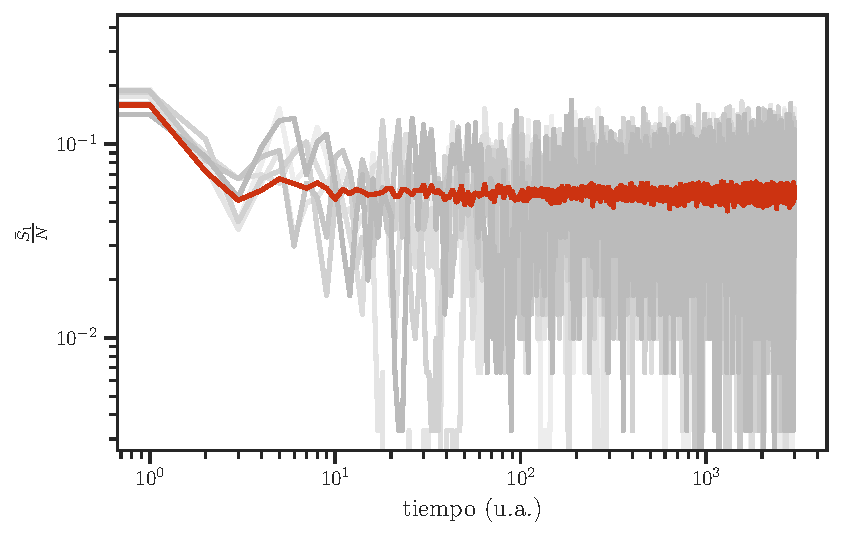
\includegraphics[width=\imsize]{transitorio.pdf}
	\caption[Parámetro de orden ($\bar{S}_1/N$ ) en función del tiempo, para 6 realizaciones  en el punto crítico, y los parámetros $r_1=$\num{1e-3}, $r_2 = 0.6$. La linea roja es un promedio sobre 100 configuraciones del sistema.]{Parámetro de orden ($\bar{S}_1/N$ ) en función del tiempo, para 6 realizaciones  en el punto crítico, y los parámetros $r_1=$\num{1e-3}, $r_2 = 0.6$. La linea roja es un promedio sobre 100 configuraciones del sistema.}\label{fig:transitorio}
\end{figure}


\subsection{Elección de los valores $r_1$ y $r_2$}

Las probabilidades $r_1$ y $r_2$  son números pequeños, $r_1,r_2\ll1$, elegidos antes del inicio de una simulación y determinan la escala de tiempo del sistema. Para escoger  los valores óptimos de estos parámetros  optamos el  criterio  de que esta elección pueda facilitar lo máximo posible la determinación del punto crítico $T_c$.     Para encontrar el valor de $r_1$  de manera   sistemática  y eficiente   se varió  el valor del  este parámetro  manteniendo fijo el  valor  de $r_2$. Dado que $r_2$ es una probabilidad que esta relacionada con el tiempo en que pasa la dinámica neuronal del sistema en el periodo refractario, se optó por tomar un valor de $r_2=0.5$, este valor nos permite  tener un balance entre el tiempo que esta en el estado  refractario y quiescente.  Para cada par $(r_1,r_2)$  se midieron los valores de $\frac{\bar{S}_1}{N}$, $\bar{S}_2$ y $\chi(T)$ promediados para $100$ configuraciones en función del umbral $T$.   El resultado se muestra en la \Cref{fig:diagrama_fase_variando_r1}. Para un valor demasiado grande     $r_1$=\num{1e-1}  la actividad neuronal  no se extingue para valores muy grandes de  $T$, esto nos sugiere que para este valor de $r_1$  la dinámica neuronal esta dominada por  la  auto-excitación  de las neuronas. Este comportamiento no es biológicamente correcto, debido a  que se espera que para grandes valores de $T$ la dinámica neuronal se extinga.  Para valores grandes de $r_1$ como  \num{1e-2}, el punto critico no se puede determinar de forma precisa debido a que los parámetros   $\left\langle\frac{\bar{S}_1}{N}\right\rangle_c, \left\langle\chi\right\rangle_c$   no poseen un máximo claro. Finalmente al bajar el valor de $r_1=$ \num{1e-4} se evidencia  que el parámetro de orden $\left\langle\frac{\bar{S}_1}{N}\right\rangle_c$ empieza con un valor finito arriba del punto crítico y llega  a un  valor cercano a cero en el punto crítico, mientras que $\left\langle\frac{\bar{S}_1}{N}\right\rangle_c$ y $\left\langle\chi\right\rangle_c$ muestran un pico en el entorno del punto crítico, tal como se espera en un fenómeno tipo percolación.\\


\begin{figure}[h!]
	\centering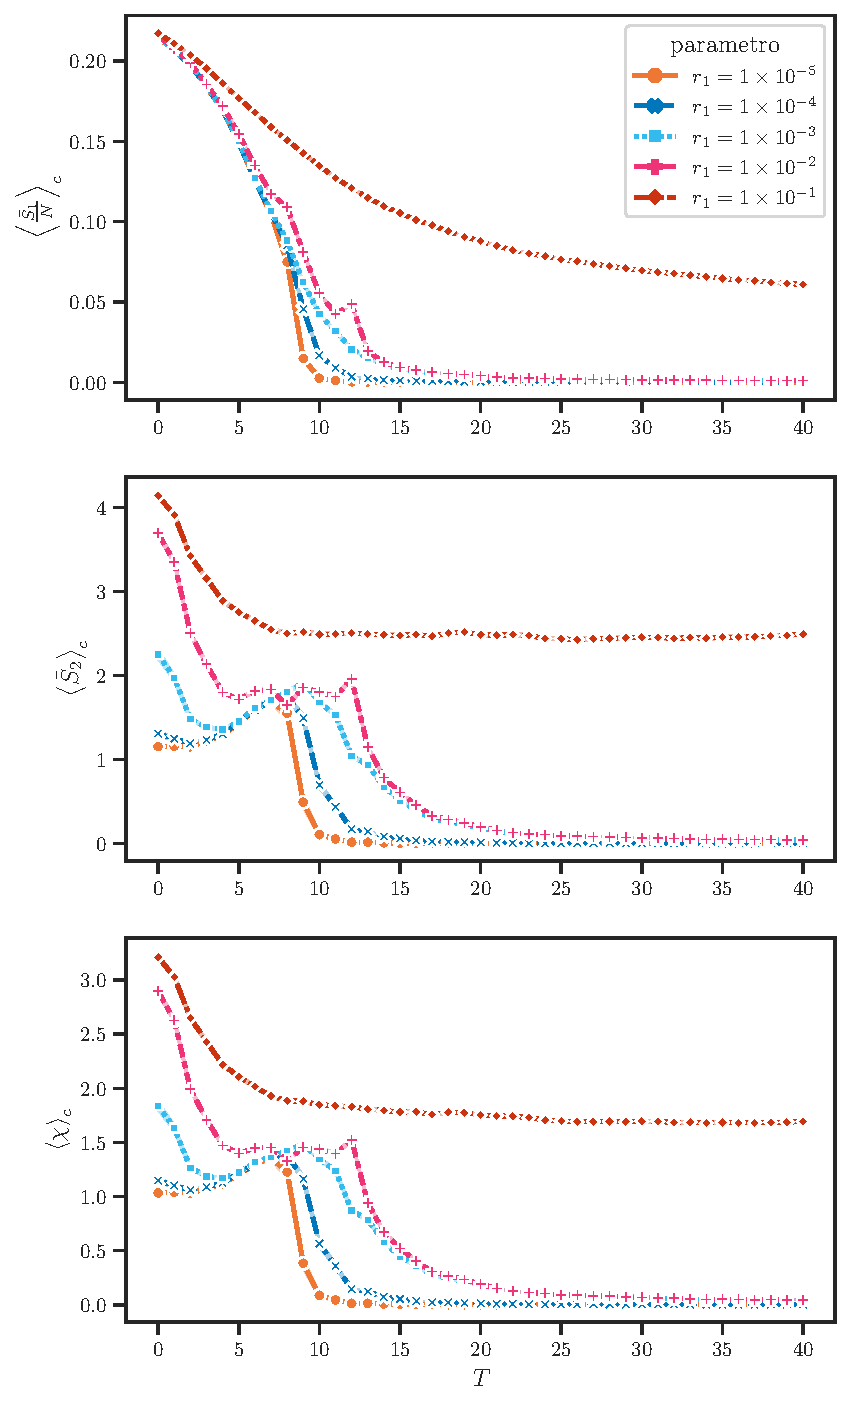
\includegraphics[width=\imsize]{variando_r1_hermafrodita.pdf}
	\caption[Comportamiento de los parámetros  que caracterizan la  dinámica neuronal   en función del parámetro de umbral $T$  para diferentes
	valores de $r_1$ manteniendo fijo el parámetro $r_2=0.5$.]{Comportamiento de los parámetros de orden que caracterizan la  dinámica neuronal   en función del parámetro de umbral $T$  para diferentes
		valores de $r_1$ manteniendo fijo el parámetro $r_2=0.5$. (a) Parámetro de orden $\left\langle\frac{\bar{S}_1}{N}\right\rangle_c$. (b) Tamaño del segundo mayor cluster $\left\langle\bar{S}_2\right\rangle_c$. (c) Tamaño promedio de los clústeres $\left\langle\chi\right\rangle_c$. Todos los parámetros fueron promediados durante $100$ configuraciones de la dinámica neuronal.}\label{fig:diagrama_fase_variando_r1}
\end{figure}



Para determinar el valor de $r_2$, se realizó el mismo procedimiento para determinar el valor de $r_1$,  es decir, para un tamaño fijo y un valor constante de $r_1$ se cambió el valor $r_2$, y se observó  el comportamiento de los tres parámetros $\left\langle\frac{\bar{S}_1}{N}\right\rangle_c$ , $\left\langle\bar{S}_2\right\rangle_c$ y $\left\langle\chi\right\rangle_c$ en función del umbral $T$ cada uno para 100 realizaciones de la dinámica neuronal . Como se ve en la \Cref{fig:diagrama_fase_variando_r2}  para un valor muy bajo de $r_2=$\num{1e-2}  el diagrama de fase no muestra un pico en los parámetros  $\left\langle\frac{\bar{S}_1}{N}\right\rangle_c$ y $\left\langle\bar{S}_2\right\rangle_c$  y el comportamiento del parámetro de orden $\left\langle\frac{\bar{S}_1}{N}\right\rangle_c$ muestra que la dinámica neuronal es cercana a $0$. Esto se debe al hecho de que  $r_2$ es la probabilidad de transición $R\to Q$  por lo tanto al ser tan baja esta probabilidad es poco probable que el sistema realice esta transición y en consecuencia el sistema pasa gran parte de su dinámica  en el estado refractario. Para los valores $r_2 = 0.2$  o $0.3$, el tamaño de los parámetros $\left\langle\frac{\bar{S}_1}{N}\right\rangle_c$ y $\left\langle\bar{S}_2\right\rangle_c$ no exhibe tanta diferencia, en cambio para los valores grandes
disminuyen significativamente y los picos de dichos valores aparecen en valores menores de
éstos parámetros. Esto significa que para los valores grandes de $r_2$ aparecen clústeres con tamaños más pequeños. En base a estos resultados, se eligió el valor $r_2 = 0.6$  en todas las siguientes simulaciones.

\begin{figure}[h!]
	\centering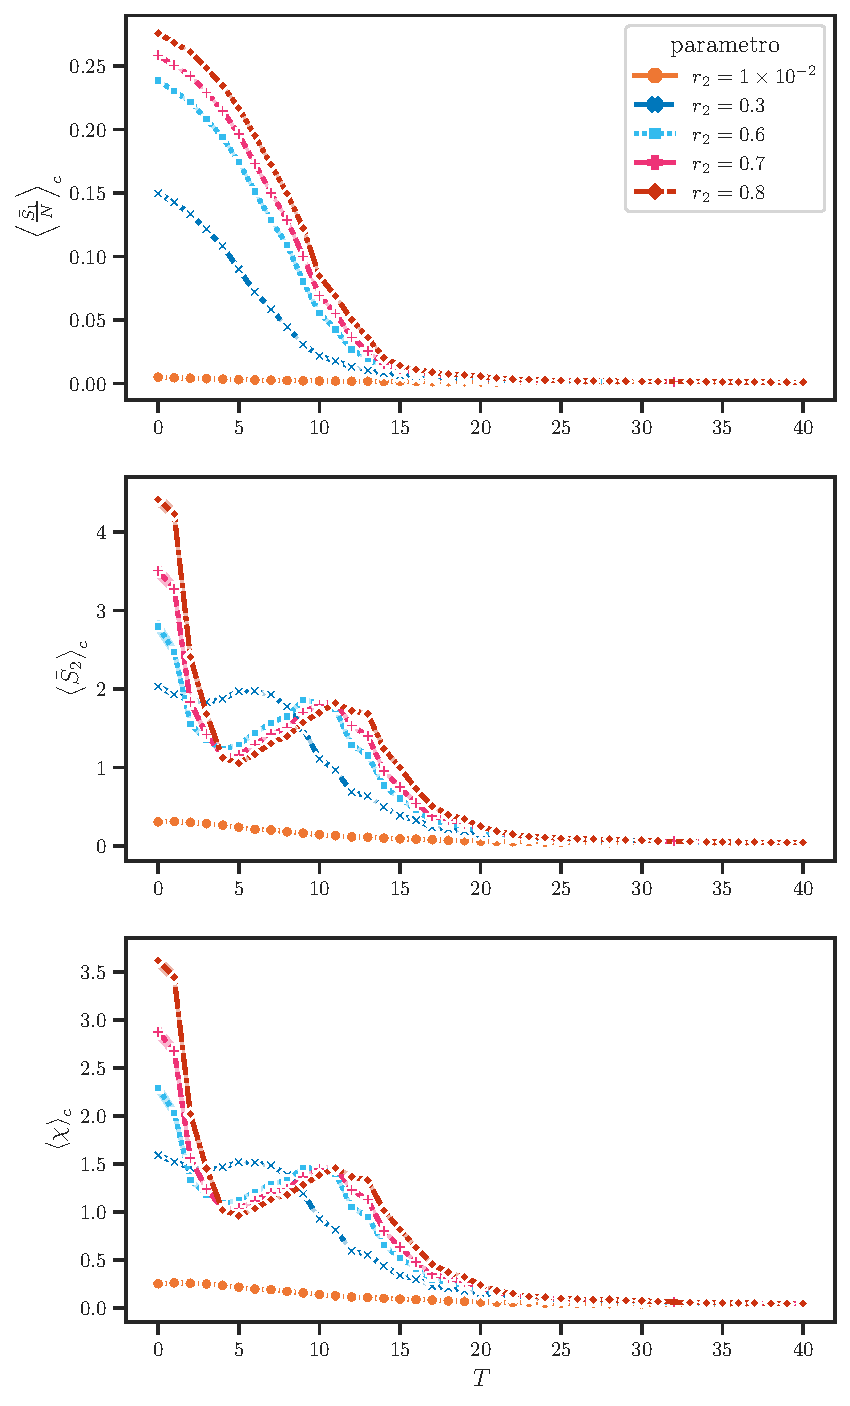
\includegraphics[width=\imsize]{variando_r2_hermafrodita.pdf}
	\caption[Comportamiento de los parámetros  que caracterizan la  dinámica neuronal   en función del parámetro de umbral $T$  para diferentes
	valores de $r_2$ manteniendo fijo el parámetro $r_1$.]{Comportamiento de los parámetros de orden que caracterizan la  dinámica neuronal   en función del parámetro de umbral $T$  para diferentes valores de $r_2$ manteniendo fijo el parámetro $r_1$. (a) Parámetro de orden $\left\langle\frac{\bar{S}_1}{N}\right\rangle_c$. (b) Tamaño del segundo mayor cluster $\left\langle\bar{S}_2\right\rangle_c$. (c) Tamaño promedio de los clústeres $\left\langle\chi\right\rangle_c$. Todos los parámetros fueron promediados durante $100$ configuraciones de la dinámica neuronal.}\label{fig:diagrama_fase_variando_r2}
\end{figure}





\section{Resultados de la  dinámica del modelo}


\subsection{Diagrama de fases}

Habiendo encontrado los parámetros $r_1$ y $r_2$ óptimos, en esta parte se  procedió  a caracterizar los distintos regímenes del diagrama de fase de la dinámica neuronal del sistema. Teniendo en cuenta los resultados anteriores para cada  configuración del sistema se fijaron  los parámetros del modelo a los siguientes valores: $r_1=$\num{1e-4}, $r_ 2 =0.6$,  $t_s = 10000$ con un transitorio de $800$ pasos de tiempo. Luego calculamos los parámetros $\left\langle   A(t) \right\rangle $,  $\sigma(A)$, $\left\langle S_1/N \right\rangle $ y $\left\langle S_2\right\rangle $, como una función del umbral $T$ en el intervalo  $[0, 40]$.  Para obtener buenas estadísticas los anteriores parámetros fueron promediados  en $100$ configuraciones del sistema, partiendo de valores de estados iniciales aleatorios. El umbral de activación $T$ es el parámetro utilizado para controlar la dinámica del sistema. Con el conectoma de cook hermafrodita como red subyacente, el modelo admite una transición de fase dinámica, y el valor crítico del umbral es $T_c\approx12$.


En la figura \Cref{fig:diagrama_fase} se ilustra el resultado de la actividad neuronal simulada promediada en $100$ configuraciones para diferentes valores de $T$, mientras se mantienen fijos $r_1$ y $r_2$.  Las franjas de color indican el intervalo de confianza con áreas iguales alrededor de la mediana de los parámetros. De acuerdo a esta figura, cada una de las  cantidades calculadas muestra un comportamiento suave en función de $T$ por tanto tal comportamiento es un fuerte indicador de una transición de fase dinámica  segundo orden o critica  en el umbral crítico $T_c$ dado por el valor correspondiente de $T$ tal como  la teoría  de percolaciónes estudiada en el \Cref{sec:Sucebtibilidad} predecía.   Como se muestra en la  \Cref{fig:diagrama_fase}a y  \Cref{fig:diagrama_fase}b  el tamaño promedio de clústeres $\left\langle \chi \right\rangle $ y el tamaño del segundo clúster  más grande $\left\langle S_2\right\rangle $, son   cantidades adecuadas para caracterizar la transición de fase y esta se encuentra cerca del máximo local (si existe el máximo) de estas cantidades. 


esta ocurre en el valor correspondiente de $T=T_c$ donde estos parámetros  son máximos.   Además  del tamaño promedio de los clústeres y del tamaño del segundo clúster, el pico en la desviación estándar, $\sigma(A)$, también se puede usar para inferir la transición crítica.   También el parámetro de orden   $\left\langle S_1/N \right\rangle $ y el promedio de la fracción de sitios activos $ \left\langle A(t) \right\rangle$     presentan  un cambio pronunciado en el punto critico.   Por el contrario, para valores pequeños del umbral de activación ($T \ll T_c$ ), el sistema se caracteriza por altos niveles de excitación, es decir, la señal de una neurona  activa se propagará fácilmente a sus neuronas postsinápticas. En este escenario, tenemos la llamada fase supercrítica o desordenada, que se caracteriza por una actividad espontánea sostenida con fluctuaciones rápidas y temporalmente no correlacionadas (\Cref{fig:actividad_activos}, serie temporal azul).  Por otro lado, valores altos de $T$ ($T \gg T_c$ ) conducen a una fase subcrítica u ordenada, que se caracteriza por una actividad regular, de propagación corta,  donde se alternan los períodos de activación y quiescencia y en donde la excitación espontánea no podía volverse autosostenida. En este caso, solo aquellas neuronas con las conexiones más fuertes determinarán el flujo de excitación en la red (\Cref{fig:actividad_activos}, serie temporal verde).  La fase crítica aparece entre estos dos estados, cuando la actividad neuronal muestra un comportamiento oscilatorio y con correlaciones temporales de largo (\Cref{fig:actividad_activos}, serie temporal roja).  En esta fase los parámetros  revelan una transición  entre una fase en la que un clúster gigante cubre aproximadamente el 15\% del sistema (mientras que el segundo clúster más grande y el tamaño promedio de los clústeres tienen un tamaño insignificante)  y otra fase en la las neuronas no logran fusionarse en grandes clústeres.    


\begin{figure}[h!]
	\centering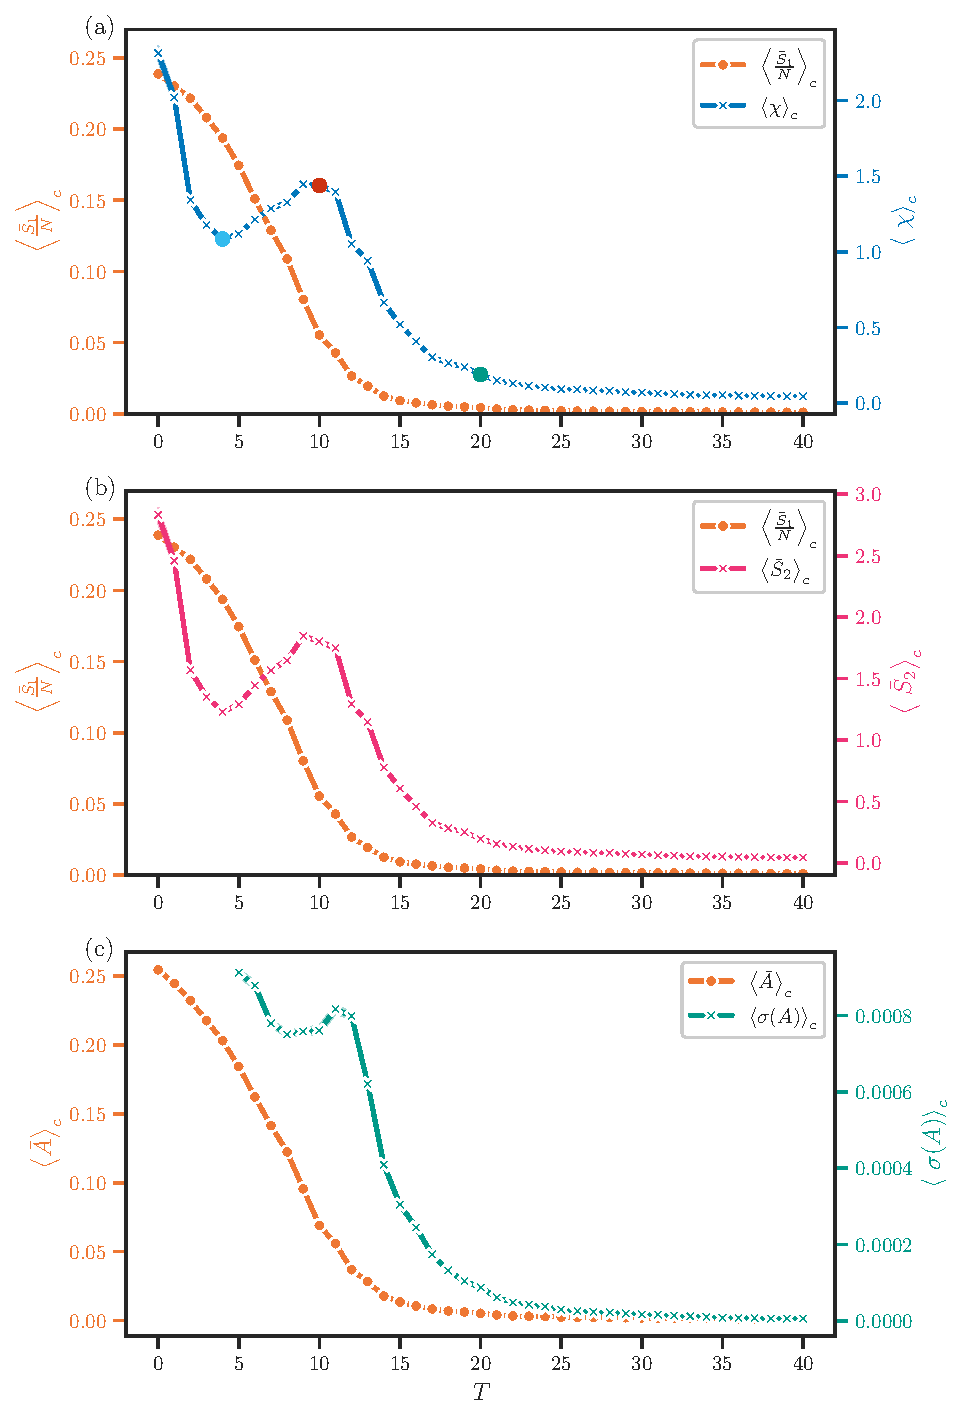
\includegraphics[width=\imsize]{diagrama_fase_hermafrodita_completo.pdf}
	\caption[Resultados del modelo de criticidad neuronal  sobre el conectoma de C. elegans hermafrodita. ]{Resultados del modelo de criticidad neuronal  sobre el conectoma de C. elegans hermafrodita. Los parámetros fueron el resultado de promediar  100 configuraciones del sistema. Las franjas de color indican el intervalo de confianza con áreas iguales alrededor de la mediana de los parámetros. (a)  muestra el tamaño del clúster gigante (es decir, el parámetro de orden, $\bar{S}_1/N$, línea naranja) y el tamaño promedio de los clústeres ($\bar{\chi}$, línea azul) en función del umbral $T$ (parámetro de control), así como el punto crítico $T_c \sim 12$. El pico en $\bar{\chi}$ (punto rojo) se identifica como la transición de fase crítica. Los puntos azules y verdes corresponden a  valores de T en la fase supercritica y subcritica respectivamente. (b)  El clúster mas grande  (linea naranja) y el tamaño del segundo clúster mas grande  (linea azul). (c)   Actividad media (línea naranja) y su desviación estándar (linea azul).  Tanto el parámetro de orden  como la actividad media muestran un cambio abrupto al rededor del punto critico $T_c$, mientras que los parámetros  $\left\langle  \chi \right\rangle$, $\left\langle S_2 \right\rangle$ y $\sigma(A)$ muestran un pico al rededor de este parámetro. }\label{fig:diagrama_fase}
\end{figure}



\begin{figure}[h!]
	\centering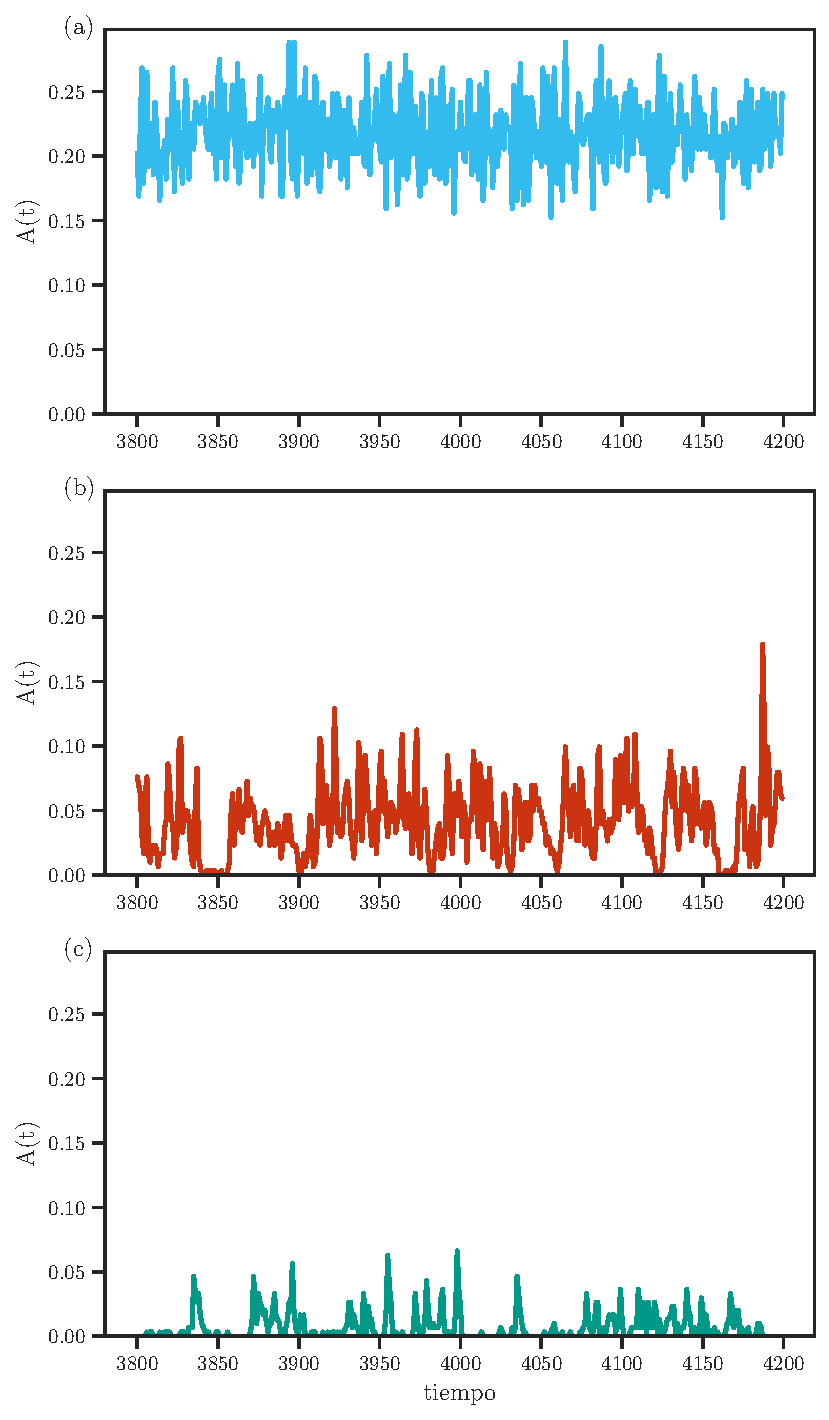
\includegraphics[width=\imsize]{actividad_activos_hermafrodita.pdf}
	\caption[Dinámica de la actividad media del sistema , $A(t) = 1/N \sum_j \delta_{s_j(t),E}$, para diferentes valores del umbral de activación $T$. ]{Dinámica de la actividad media del sistema, $A(t) = 1/N \sum_j \delta_{s_j(t),E}$, para diferentes valores del umbral de activación $T$; la fase supercrítica $T \ll Tc$ (serie temporal azul), la fase crítica $T = T_c$ (rojo) y la fase subcrítica $T \gg Tc$ (verde). }\label{fig:actividad_activos}
\end{figure}



En la \Cref{fig:probabilidad} mostramos ejemplos de la propagación espacio-temporal de la actividad a partir de una configuración de estados iniciales aleatorios. El eje vertical indexa las neuronas de la red (ordenados por tiempo de primera activación) y en el eje horizontal se codifica la evolución temporal. El código de colores representa la probabilidad de que una neurona  se active sobre un total de 100 simulaciones independientes. Es evidente que un umbral de propagación bajo dio como resultado una  actividad neuronal que decae rápidamente. Un umbral de propagación alto resultó en una probabilidad muy alta de observar neuronas activadas en cualquier momento. Finalmente, el umbral crítico $T_C$ permitió una actividad autosostenida con niveles intermedios de actividad después del estado inicial. 



\begin{figure}[h!]
	\centering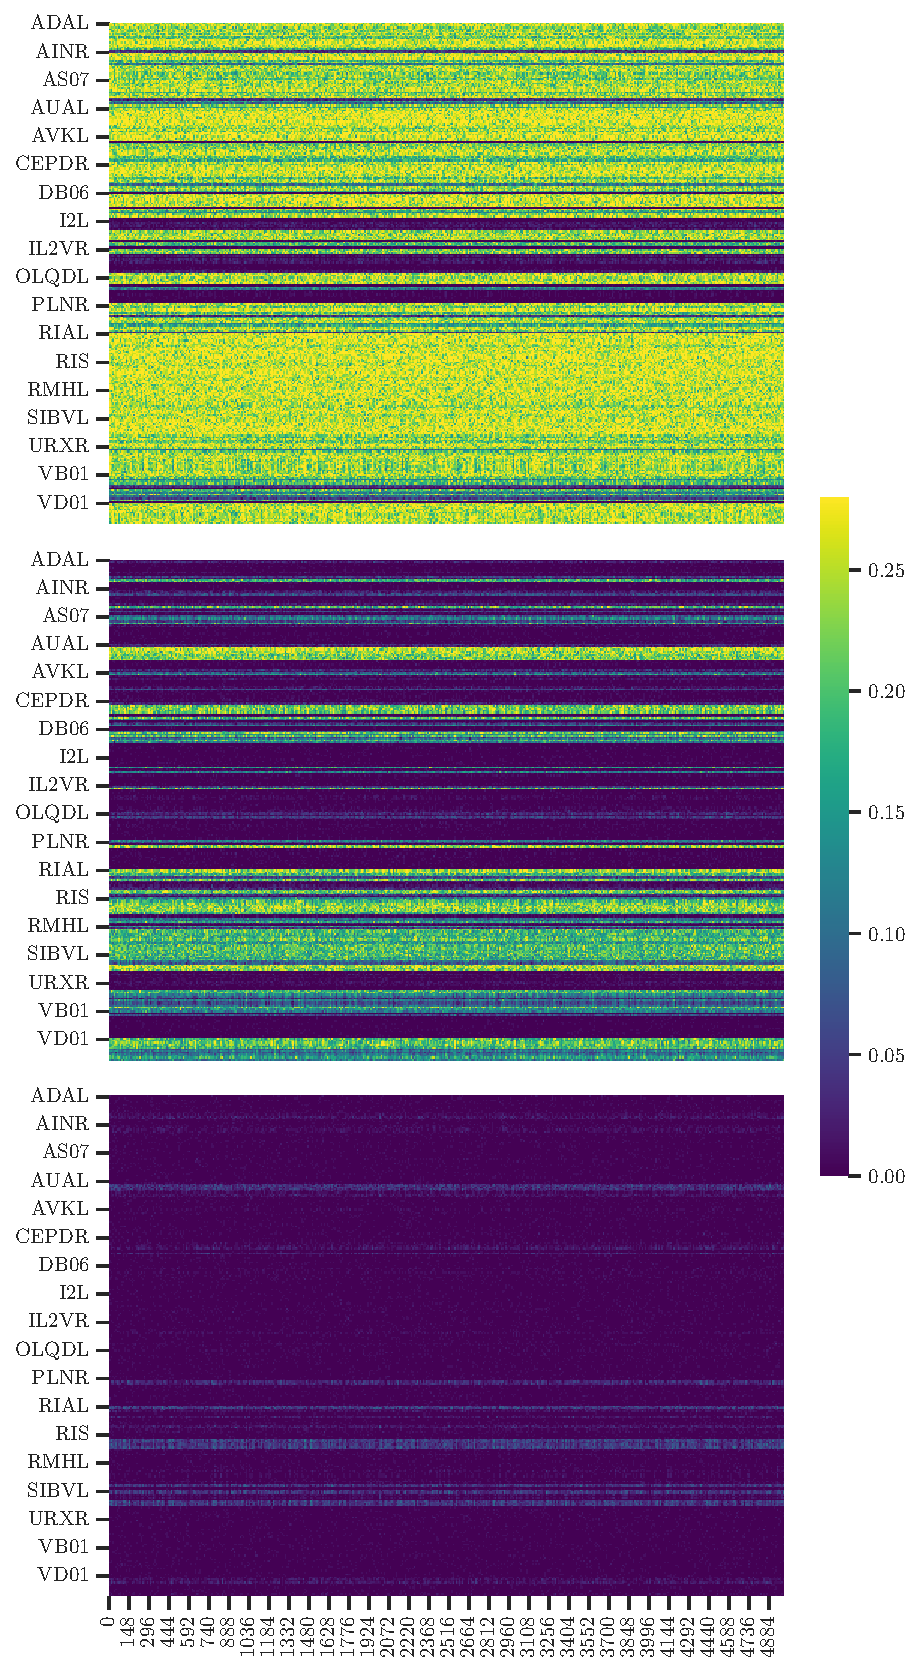
\includegraphics[width=\imsize]{probabilidad_hermafrodita.pdf}
	\caption[Probabilidad de observar activaciones de neuronas (100 simulaciones independientes) en función del tiempo para tres umbrales diferentes .]{Probabilidad de observar activaciones de neuronas (100 simulaciones independientes) en función del tiempo para tres umbrales diferentes.}\label{fig:probabilidad}
\end{figure}


Otra forma de caracterizar el sistema es  analizar como varia para cada valor de $T$ las fracciones de sitios excitados, refractarios y quiescentes.  Es importante recordar que como estos 3 parámetros son probabilidades en cada valor de $T$ se cumple la relación $\bar{Q} + \bar{A} +\bar{R} = 1$.  El resultado se muestra en la \Cref{fig:fraccion_sitios}. El comportamiento de la fracción de sitios quiescentes $\bar{Q(t)}$ es del tipo de una curva de crecimiento logístico  donde esta muestra una progresión  desde unos niveles bajos al inicio, hasta acercarse a un punto de inflexión para un cierto valor de $T$ que coincide con el punto critico $T_c$; la transición se produce en una región caracterizada por una fuerte aceleración intermedia hasta que para valores muy grandes de ($T \gg T_c$)  la curva  se satura hasta probabilidad cercana a 1 de permanecer en el estado quiescente, es decir la actividad neuronal se extingue.  Por otro lado La fracción  de sitios activos $\bar{A(t)}$ y refractarios $\bar{R(t)}$ disminuyen monótonamente a medida que la fraccion de sitios quiescentes  $\bar{Q(t)}$ aumenta monótonamente. Tanto la fracción de sitios activos $\bar{A(t)}$ y refractarios $\bar{R(t)}$ tienen un punto de inflexión al igual que   $\bar{Q(t)}$ en el punto critico.



\begin{figure}[h!]
	\centering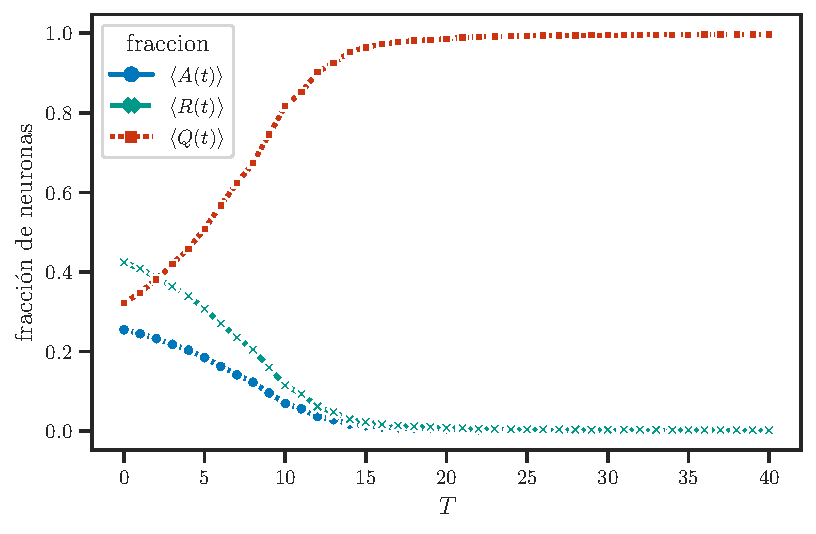
\includegraphics[width=\imsize]{fraccion_de_sitios.pdf}
	\caption[Fracción de sitios activos, refractarios y quiescentes en función del parámetro de control $T$ promediados en  100 configuraciones del sistema .]{Fracción de sitios activos, refractarios y quiescentes en función del parámetro de control $T$ promediados en  100 configuraciones del sistema.}\label{fig:fraccion_sitios}
\end{figure}



Finalmente se compararon  las predicciones de campo medio del punto crítico  dadas en el \cref{sec:campomedio} con los resultados de las simulaciones del modelo.  Para el conectoma hermafrodita  el valor de la fuerza media de la red es $\left\langle W \right\rangle = \sum_i W_i/N=69.42052$ .  Sustituyendo el valor de $\left\langle W \right\rangle $  y los valores de $r_1$ y $r_2$ en la \cref{eq:78} obtenemos la predicción de la probabilidad probabilidad de que la neurona  esté excitada,  en estado quiescente,  o en estado refractario  y el valor del punto crítico mediante el campo medio.


\begin{equation}\label{eq:79}
	\begin{aligned}
		T_c & \approx 18.93 ,	\\
		\bar{p}&=\bar{A(t)}= \eqqcolon p_{-} \approx 0.2727 &\ \text{cuando} \ T<T_c \\
		\bar{p} &= r_1\bar{q} = \frac{r_1r_2}{r_1+r_2+r_1r_2}\eqqcolon p_{+}  \approx \num{9.9973e-5} &\ \text{cuando} \ T>T_c\\
	\end{aligned}
\end{equation}

Los resultados de las simulaciones nos arrojan un valor de  $\bar{p}=\bar{A(t)}=0.247=p_{-}$, $\bar{q} = 0.34$ cuando $T<T_c$ y $\bar{p}=\bar{A(t)}=0.0006965$, $r_1\bar{q} = \num{9.98e-5}$  cuando $T>T_c$, estos resultados son muy cercanos a los predichos. Como era de esperar, $p_{+} < p_{-}$, lo que implica que la actividad es alta cuando el umbral es bajo. Por otro lado el valor de $T_c$ es mucho mas alejado de lo esperado, esto se debe a que el sistema tiene un valor de $N$ muy pequeño y la aproximación de campo medio es mas fiable cuando $N\to\infty$.




\section{Clústeres de actividad neuronal }\label{sec:actividad_neuronal_modelo}

En este apartado, caracterizamos los patrones espaciales de la actividad neuronal colectiva calculando el número de clústeres y su distribución de tamaños  en el modelo de dinámica neuronal para posteriormente comparar sus resultados  con lo obtenido en los datos experimentales (\Cref{sec:actividad_neuronal_experimento}).  

\subsection{Correlación entre actividades neuronales }\label{sec:correlacion_modelo}


Para visualizar  los grupos de neuronas que comparten actividad en  las series temporales, se aplicó a la actividad neuronal simulada (una sola realización del sistema)  un algoritmo de clustering jerárquico a las tres  regiones  del diagrama de fase (súper-crítico: $T<T_c$; crítico: $T=T_c$ y sub-critico: $T>T_c$ ).  En la región súper-critica (\Cref{fig:cluster_supercritico}) la actividad neuronal es aleatoria y no existen clústeres de neuronas sincronizadas. Esto se ve evidenciado al  calcular el coeficiente de correlación de Pearson  por pares de neuronas a la dinámica neuronal, dando como resultado correlaciones cercanas a cero. Como evidencia de lo  anterior, dos neuronas con una actividad neuronal  espontanea muy similar en los datos experimentales  ( (AVAL, AVAR), cuyo  coeficiente de correlación en los datos de Kato et al. es 0.969 ) tienen un coeficiente de correlación de -0.015, lo que nos sugiere que no existe correlación alguna en este par de neuronas, lo que contradice a los datos experimentales.  


Por otro lado, en la región sub-critica  (\Cref{fig:cluster_subcritico})   la dinámica neuronal esta limitada a pocas neuronas y los coeficientes de correlación entre neuronas distantes  son prácticamente cero.  Lo que nos sugiere que la dinámica neuronal se limita a  neuronas cercanas con conexiones fuertes.  Finalmente, el comportamiento mas rico y complejo de la actividad neuronal simulada  se encuentra al rededor del punto critico (\Cref{fig:cluster_critico}). Mostrando  grupos de neuronas  que tienen  activación e inactivación sincronizadas tal como los datos experimentales (\Cref{fig:seriedatos}). Al determinar las correlaciones cruzadas en las actividades neuronales (\Cref{fig:correlacion_critico}) encontramos algunos de los grupos  bien conocidos de neuronas relacionadas con los movimientos de retroceso y avance tal como los encontramos en los datos experimentales ([AVA, AVE,  RIM], [RIB,RID y RME] ). 



\begin{figure}
	\centering
	\begin{subfigure}[b]{0.3\textwidth}
		\centering
		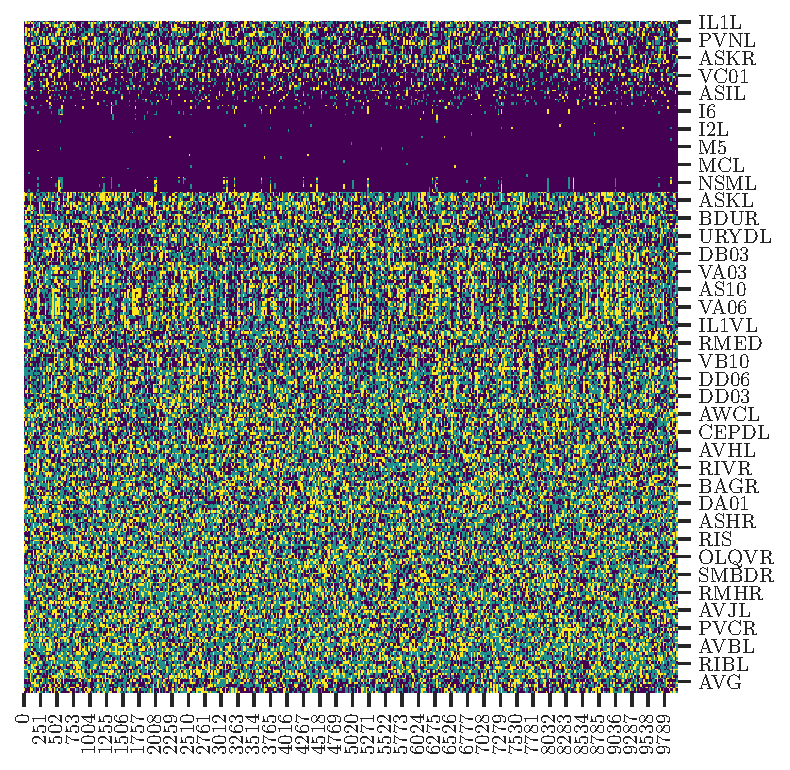
\includegraphics[width=\textwidth]{cluster_super_critico}
		\caption{}
		\label{fig:cluster_supercritico}
	\end{subfigure}
	\begin{subfigure}[b]{0.3\textwidth}
		\centering
		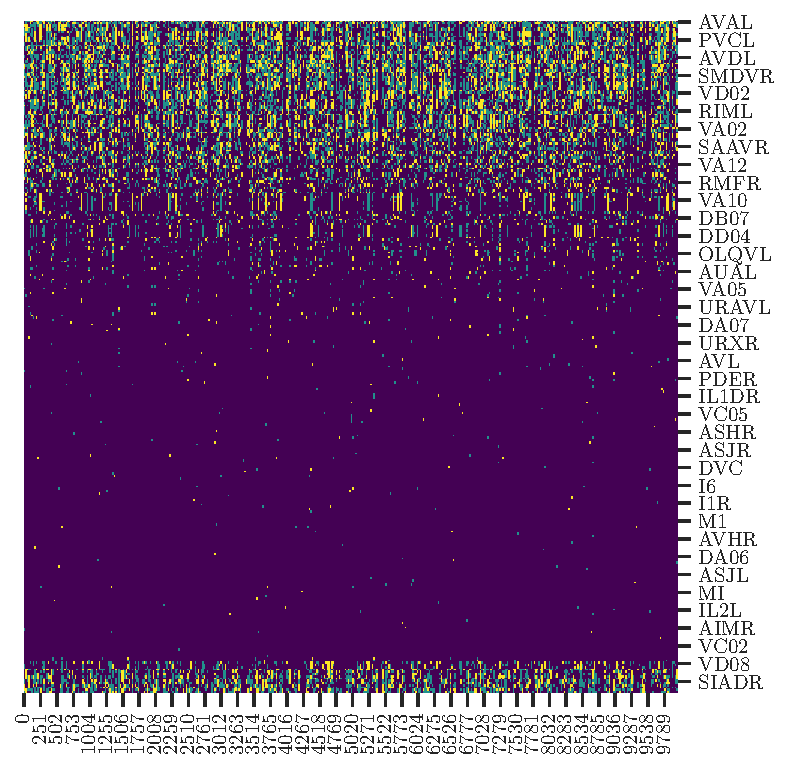
\includegraphics[width=\textwidth]{cluster_critico}
		\caption{}
		\label{fig:cluster_critico}
	\end{subfigure}
	\begin{subfigure}[b]{0.3\textwidth}
		\centering
		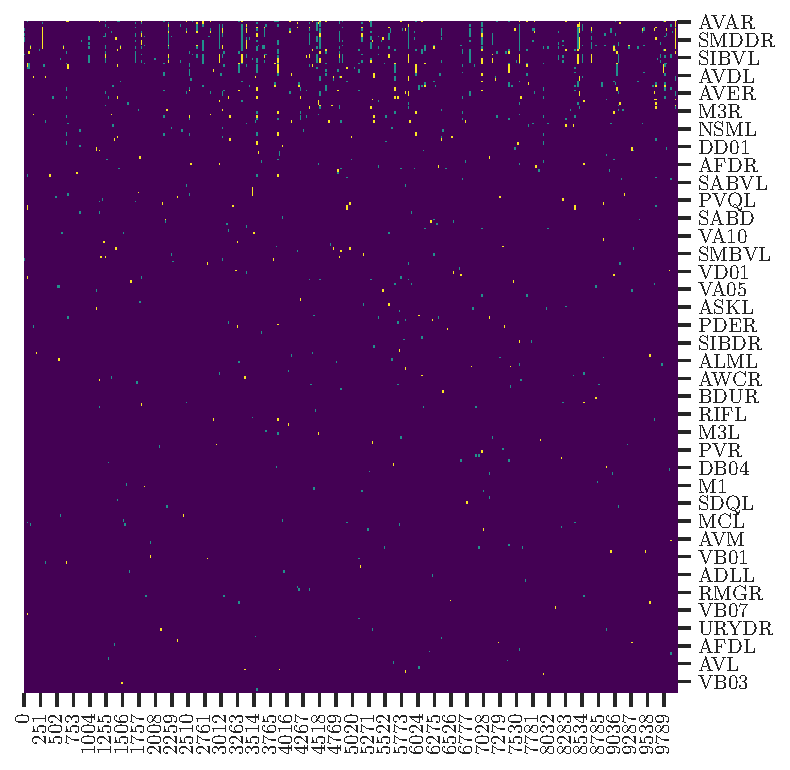
\includegraphics[width=\textwidth]{cluster_sub_critico}
		\caption{}
		\label{fig:cluster_subcritico}
	\end{subfigure}
	\caption[Serie temporal de la actividad de las neuronas simuladas en las tres regiones distintas del diagrama de fase del para una realización del modelo de criticidad neuronal.]{ Serie temporal de la actividad de las neuronas simuladas en las tres regiones distintas del diagrama de fase para una realización  del modelo de criticidad neuronal. Cada fila representa una neurona, cuyo orden se determinó mediante agrupamiento jerárquico. (a) Región súper-crítica  (b) Región critica (c) Región sub-crítica. En los diagramas el color amarillo se corresponde al estado excitado ($s=1$), el azul al  quiescente ($s=0$) y el verde al refractario ($s=0.5$). }\label{fig:series_simulacion}
\end{figure}



\begin{figure}[h!]
	\centering
	\begin{subfigure}[b]{0.3\textwidth}
		\centering
		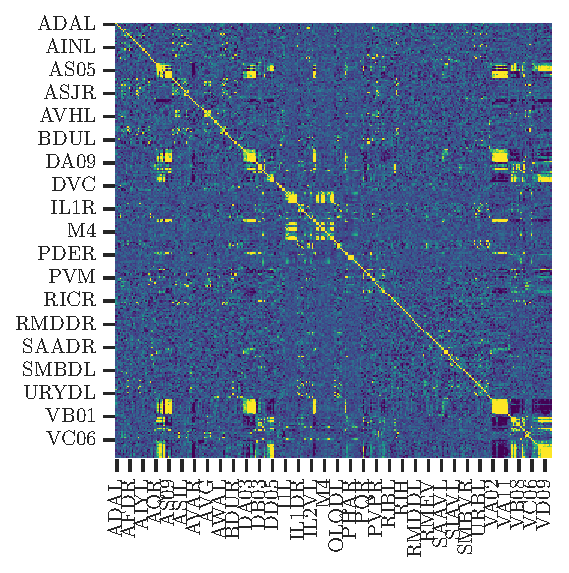
\includegraphics[width=\textwidth]{correlacion_super_critico.pdf}
		\caption{}
		\label{fig:correlacion_super_critico}
	\end{subfigure}
	\begin{subfigure}[b]{0.3\textwidth}
		\centering
		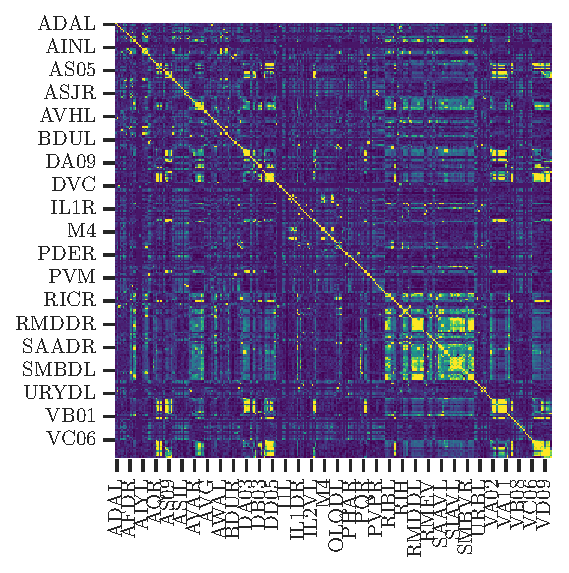
\includegraphics[width=\textwidth]{correlacion_critico.pdf}
		\caption{}
		\label{fig:correlacion_critico}
	\end{subfigure}
	\begin{subfigure}[b]{0.3\textwidth}
		\centering
		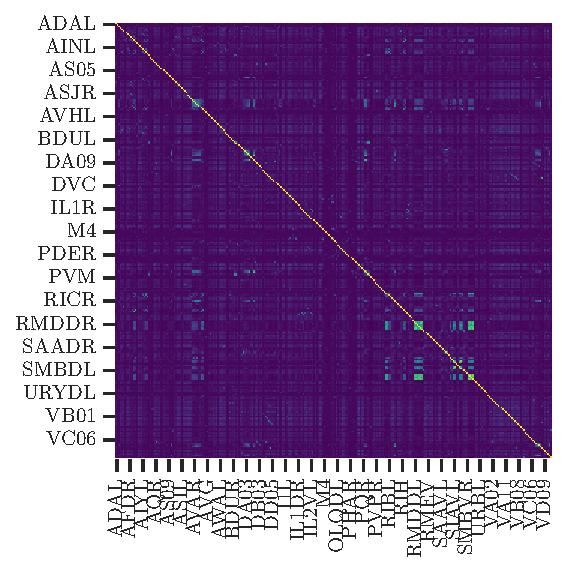
\includegraphics[width=\textwidth]{correlacion_sub_critico.pdf}
		\caption{}
		\label{fig:correlacion_sub_critico}
	\end{subfigure}
	\caption[ Correlación cruzada por pares de las actividades de las neuronas simuladas  en las tres regiones del diagrama de fase para para una realización del sistema del modelo de criticidad neuronal.]{ Correlación cruzada por pares de las actividades de las neuronas simuladas  en las tres regiones del diagrama de fase para para una realización del sistema del modelo de criticidad neuronal. (a) Región súper-crítica  (b) Región critica (c) Región sub-crítica. El color amarillo muestra una correlación positiva y el color azul muestra una correlación negativa.} \label{fig:correlaciones_modelo}
\end{figure}


Finalmente,  la matriz de correlación  puede verse como una forma de etiquetar los clústeres con actividad coherente, por lo que en el régimen más ordenado ($T>T_c$) todo el cerebro está activo y se fusiona en un solo grupo  activado, mientras que en el más desordenado ($T<T_c$), cada región del cerebro actúa de forma independiente. Es solo en la criticidad ($T_c$) donde son posibles clústeres coherentes de todos los tamaños, optimizando así el equilibrio integración/segregación.


\subsection{Estadísticas de los clústeres de la actividad neuronal }\label{eq:estadistica_clusteres_modelo}



Ahora se compararan  las estadísticas de los clústeres de la actividad neuronal  de los  datos experimentales (\Cref{eq:estadistica_cllusteres})  con las de la   dinámica neuronal del modelo en la región cercana al  punto criticó (\Cref{fig:estadisticas_clusteres_modelo}).   En primer lugar,  calculamos la relación entre $\left\langle A(t) \right\rangle$ y $m$ encontrando  que el número de clústeres alcanzaba su máximo cuando $ \left\langle A(t) \right\rangle \approx 8\%$,  un valor cercano al de los datos experimentales. El modelo revela que estas activaciones aparecen espontáneamente en el estado de reposo, sino que también muestra su relación con el régimen dinámico: orden significa una coactivación (integración) compartida de los procesos subyacentes a estos clústeres, desorden significa una segregación aumentada. En el medio, el punto de transición posiblemente represente un equilibrio óptimo de segregación/integración. También corresponde al punto en el que el cerebro muestra la mayor variabilidad en su repertorio de estados, como lo demuestra un pico en la variabilidad del parámetro $m$  frente  a este nivel de activación


En segundo lugar, calculamos la relación entre $\left\langle A(t) \right\rangle$ y el tamaño normalizado del clúster más grande.  Tal como en los datos experimentales $\bar{S}_1$  se comporta como un parámetro de orden $\left\langle A(t) \right\rangle$  y abarca un amplio rango de escalas, desde unas pocas neuronas hasta una gran proporción del cerebro (\Cref{fig:mvsfrac_modelo}(b)), solo en niveles intermedios de actividad su varianza es alta (\Cref{fig:mvsfrac_modelo}(c)). En tercer lugar, se encontró  la distribución de $\left\langle A(t) \right\rangle$ , denotada como $p(\left\langle A(t) \right\rangle)$ utilizando el histograma de los datos neuronales de la simulación, el nivel de activación espontánea estaba por debajo de $\left\langle A(t) \right\rangle_c$, y practicante no existen los eventos en donde  $p(\left\langle A(t) \right\rangle)$ era mayor que  $p(\left\langle A(t) \right\rangle)_c$ (\Cref{fig:distactivos_exp}). 


\begin{figure}[h!]
	\centering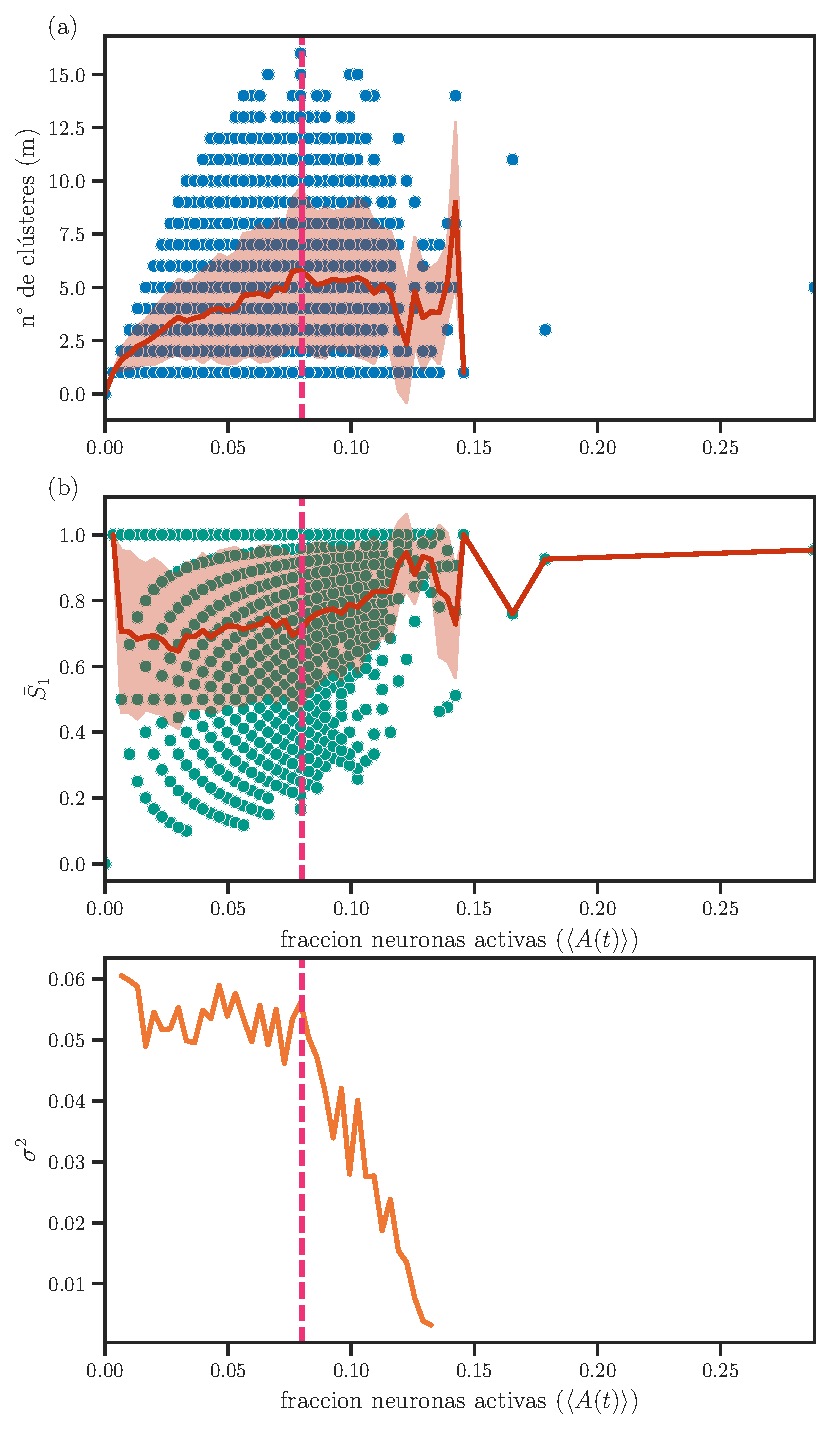
\includegraphics[width=\imsize]{estadisticas_clusteres_modelo.pdf}
	\caption[ El nivel de actividad cerebral fluctúa continuamente por encima y por debajo de una transición de fase solo en el punto critico.] {El nivel de actividad cerebral fluctúa continuamente por encima y por debajo de una transición de fase solo en el punto critico.  (a) Número de clústeres ($m$) en función de la proporción de neuronas activas ($\left\langle A(t) \right\rangle$) para la actividad neuronal simulada cercana al punto critico. Línea roja, es la media de $m$; área roja, su desviación estándar.  (b)   El parámetro de orden, definido aquí como el tamaño (normalizado) del clúster más grande, se representa en función de la fracción de sitios activos $\left\langle A(t) \right\rangle$ ( los promedios se representan con la curva roja).   (c) La varianza del parámetro de orden ($\sigma$) aumenta como se espera para una transición de fase. Ademas se observa que el pico de $\sigma$ en este panel coincide con el pico del número de clusteres $m$  en  (a). } \label{fig:estadisticas_clusteres_modelo}
\end{figure}




\begin{figure}[h!]
	\centering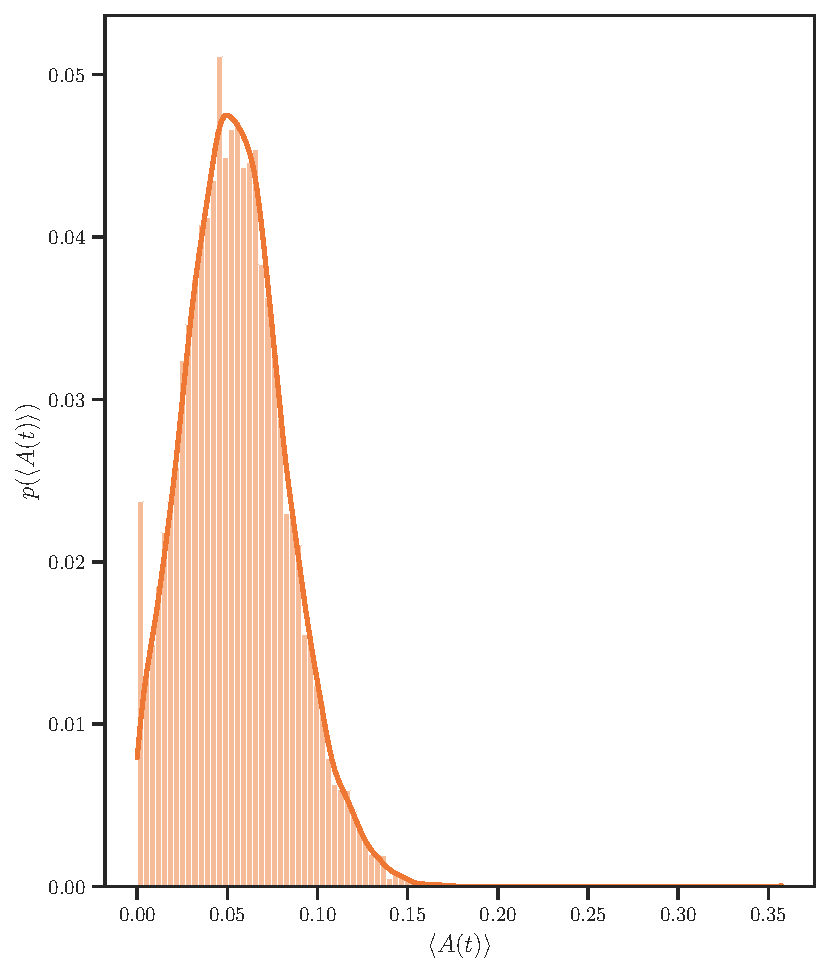
\includegraphics[width=\imsize]{fig_distactivos_modelo.pdf}
	\caption[Distribución de $p(\left\langle A(t) \right\rangle)$    de la dinámica neuronal simulada cercana al punto critico.]{Distribución de $p(\left\langle A(t) \right\rangle)$    de la dinámica neuronal simulada cercana al punto critico.. Se calculo también la KDE de cada distribución.} \label{fig:distactivos_exp}
\end{figure}

Finalmente como prueba de que los   grupos de neuronas que pertenecen a un mismo clúster presentan  un patrón de actividad similar, se realizo una  inspección visual de su sincronización y posteriormente se   calculó el correlograma mediante  RWTLCC de la dinámica neuronal simulada.  El resultado se muestra en la \Cref{fig:correlaciones_clusteres_modelo}.  Cuando las neuronas pertenecen al mismo clúster (señales azules y naranjas en la \Cref{fig:correlaciones_clusteres_modelo})  tanto la inspección visual como el correlograma muestran una similitud temporal entre estos dos  pares de neuronas. Por el contrario si no hacen parte del mismo clúster (señales verdes y rosadas)  no  existe esta similitud. 

\begin{figure}[h!]
	\centering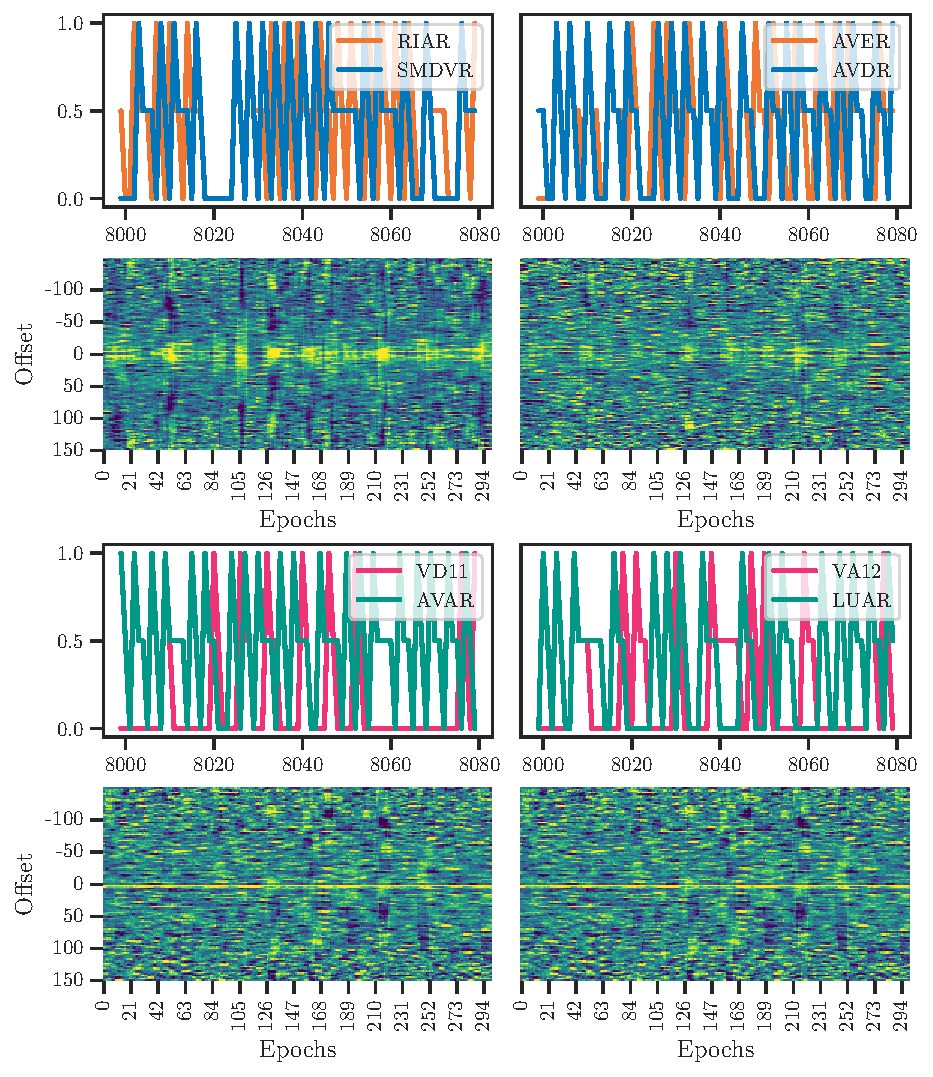
\includegraphics[width=\imsize]{correlaciones_modelo.pdf}
	\caption[Prueba de dependencias estadísticas en la actividad neuronal simulada de dos pares de neuronas que pueden hacer parte o no de un mismo clúster.]{Prueba de dependencias estadísticas en la actividad  neuronal simulada de dos pares de neuronas que pueden hacer parte o no de un mismo clúster.   Se muestra tanto la   inspección visual de sincronización entre las dos neuronas y el  correlograma del algoritmo  RWTLCC aplicado a la  dinámica neuronal.  Las señales azul y naranja pertenecen a un mismo clúster mientras que las señales verde y rosado no hacen parte del mismo clúster.  } \label{fig:correlaciones_clusteres_modelo}
\end{figure}





\subsection{Distribución del tamaño de clústeres $n(s,p)$}\label{sec:distribucion_tamaño_modelo}

Otra firma de la criticidad en el sistema es la distribución de tamaños de clústeres, $p(S)$. como se discutió en el \cref{sec:distribucion_tamaño} el  cerebro forma clústeres de actividad cuyos tamaños siguen una distribución de ley de potencia truncada, es decir, $p(s) \sim s^{-\tau}\exp\left(-s\gamma\right)$, con el cut-off exponencial debido al tamaño finito ( $\gamma \propto 1/ N$ ). Para identificar el punto crítico del sistema, calculamos la distribución de tamaños de clústeres para algunos valores de $T$, incluidos los correspondientes a los picos de $\left\langle\chi\right\rangle_c$ y $\left\langle\bar{S}_2\right\rangle_c$ (véanse la \Cref{fig:diagrama_fase}).  La gráfica resultante se muestra en la \Cref{fig:cerca_a_T_c}. Dado que la gráfica es doblemente logarítmica, una línea recta corresponde a un comportamiento de tipo ley de potencia. Vemos que a medida que el valor del parámetro $T$ se acerca a los máximos de  $\left\langle\chi\right\rangle_c$ y $\left\langle\bar{S}_2\right\rangle_c$, la distribución de tamaños de clústeres  se acerca cada vez más a un comportamiento de tipo de ley de potencia. Para un valor de $T$ que está lejos de estos picos ($T>12$), la curva $n(s, p)$ sigue el comportamiento de ley de potencia durante algún tiempo, pero luego se desvía al caer rápidamente. Este es un efecto del tamaño característico del clúster. Las distribuciones que se corresponden mas con un comportamiento de tipo de ley de potencia  son las correspondientes a los puntos $T=10$, $T=11$ y $T=12$. 

\begin{figure}[h!]
	\centering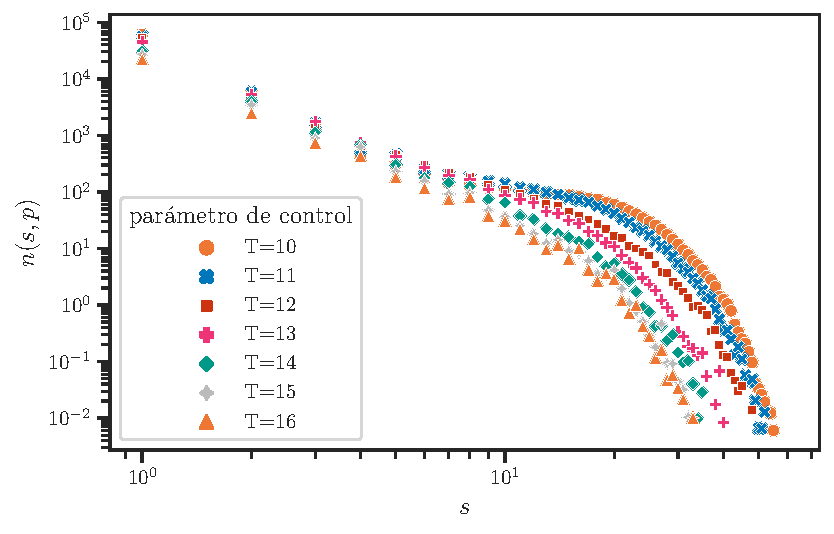
\includegraphics[width=\imsize]{cerca_a_T_c.pdf}
	\caption[Distribución de tamaño de clústeres  $n(s, p;)$ en función de $s$ para varios valores de $T$ cercanos  a los máximos de $\left\langle\chi\right\rangle_c$  y $\left\langle\bar{S}_2\right\rangle_c$.   ]{Distribución de tamaño de clústeres  $n(s, p;)$ en función de $s$ para varios valores de $T$ cercanos  a los máximos de $\left\langle\chi\right\rangle_c$  y $\left\langle\bar{S}_2\right\rangle_c$.    } \label{fig:cerca_a_T_c}
\end{figure}


Como ya se ha mencionado, la distribución de tamaños de los clústeres de actividad puede ser informativa de los diferentes regímenes dinámicos del modelo. Calculamos estas medidas en función del umbral $T$ para las tres regiones del diagrama de fase.  Las distribuciones de tamaños de clústeres se muestran en la \Cref{fig:comparacion_modelo_experimento} y se comparan con la distribución empírica obtenida en  los experimentos de Yemini et al (\Cref{fig:ley_potencia_experimentos}).   En el régimen subcrítico $T > T_c$ todos los clústeres son finitos y la distribución de los  tamaños de los clústeres tiene una cola que decae exponencialmente. En el régimen supercrítico $T < T_c$ , donde existen clústeres de gran tamaño  con probabilidad 1, la distribución tiene una cola que decae más lentamente que una exponencial. Sin embargo, cerca del punto crítico $ T\sim  T_c$, muchas cantidades se anulan o divergen exhibiendo un escaleo de tipo ley de potencia.  Solo en este punto, la distribución $n(s,p)$ del modelo, coincide con los resultados experimentales.    La distribución del tamaño de los clústeres en los datos biológicos se ajusta a una ley de potencias con un exponente de $2.15$. Esto significa que la mayoría de los clústeres son pequeños, pero hay una cola larga de clústeres grandes. La distribución del tamaño de los clústeres en los datos simulados se ajusta a una ley de potencias truncada con un exponente  $\tau = 2.22$ muy cercano al de los datos experimentales.  


Para realizar algunas comparaciones de como varia el exponente $\tau$ para  valores del parámetro de control cercanos al punto critico, aplicamos el método de MLE   a la distribución de clústeres del modelo con tres valores de $T$ distintos. Los $\tau$ calculados y su coeficiente de bondad de ajuste  tienen un valor de  ($\tau=2.4780, p=0.428$), ($\tau=2.28, p=0.912$), ($\tau=1.3450, p=0.242$) para $T=10$, $T=11$ y $T=12$ respectivamente. En todos los casos la bondad del ajuste, supera la hipótesis $H_0$ de que la distribución sigue una ley de potencias. Curiosamente en el caso de $T=12$, el modelo seguía una ley de potencias truncada con un exponente crítico $\tau$ cercano al exponente característico de los tamaños de avalanchas, $\tau = 3/2$. 


\begin{figure}[h!]
	\centering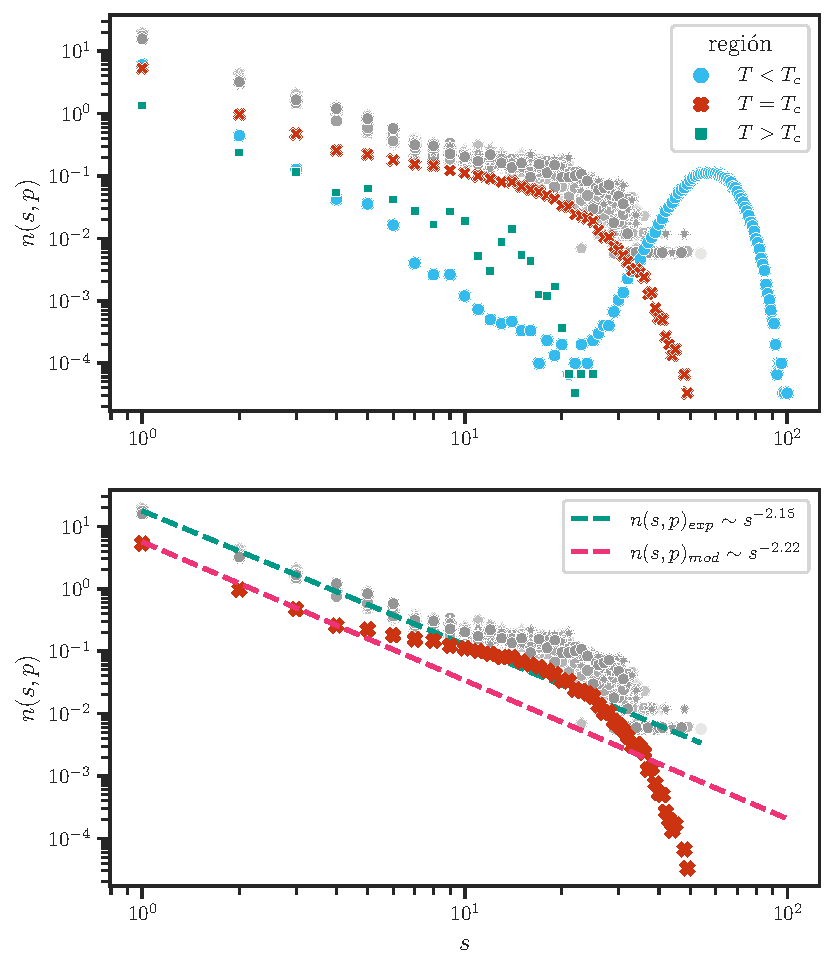
\includegraphics[width=\imsize]{comparacion_modelo_experimento.pdf}
	\caption[Distribución de tamaño de clústeres  $n(s, p;)$ en función de $s$ para varios valores de $T$  de distintas regiones del diagrama de fase.  ]{cercanos  a los máximos de $\left\langle\chi\right\rangle_c$  y $\left\langle\bar{S}_2\right\rangle_c$. La distribución de tamaños de clústeres en el umbral crítico ($T_c$) coincide con la que se observa experimentalmente. La única diferencia está en el corte de la caída de la ley de potencias, dado por la resolución más gruesa del modelo. En el régimen supercrítico ($T < T_c$) la distribución muestra la presencia de un clúster gigante, y el régimen subcrítico ($T >T_c$) solo muestra unos pocos clústeres compuestos por unos pocos nodos.} \label{fig:comparacion_modelo_experimento}
\end{figure}

 \subsection{Longitud de correlación}
 
  Al aplicar el algoritmo que calcula $g(r,p)$ junto con la distancia del camino mas corto a los distintas regiones del modelo  obtenemos la \Cref{fig:correlacion_experimento_gusano}.   Encontramos que solo en la criticidad existe  la presencia de correlaciones funcionales de largo alcance entre las neuronas.   Las correlaciones  de largo alcance son un sello distintivo de los sistemas complejos en criticidad, que se caracterizan por dinámicas espaciotemporales colectivas emergentes no triviales.   Al comparar con los datos experimentales, encontramos que los resultados se corresponden solo en el punto critico.
  

\begin{figure}[h!]
	\centering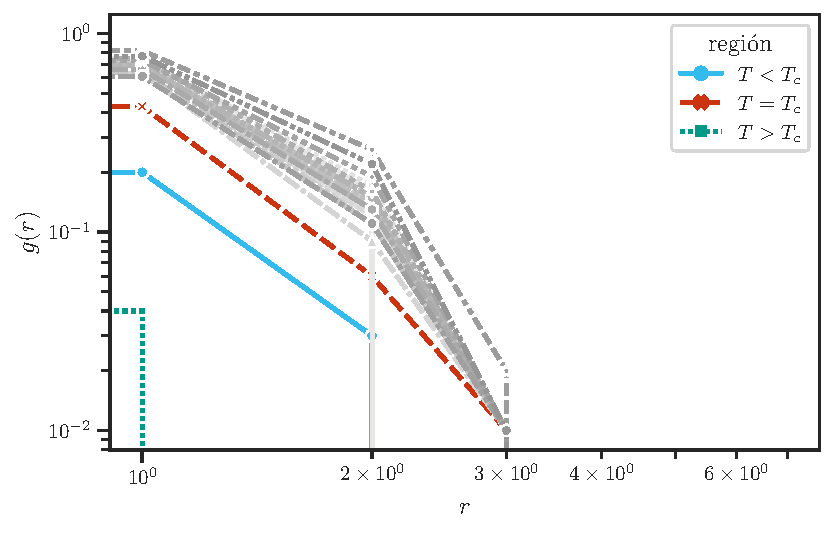
\includegraphics[width=\imsize]{correlacion_experimento_gusano.pdf}
	\caption[Función de correlación $g(r)$: en función de $r$ para varios valores de $T$  de distintas regiones del diagrama de fase.  ]{cercanos  a los máximos de $\left\langle\chi\right\rangle_c$  y $\left\langle\bar{S}_2\right\rangle_c$. La función de correlación $g(r)$ en el umbral crítico ($T_c$) coincide con la que se observa experimentalmente.} \label{fig:correlacion_experimento_gusano}
\end{figure}

Al calcular la distancia cuadrada promedio entre dos nodos $i$ y $j$ que pertenecen al mismo clúster mediante las \Cref{eq:17,eq:18} obtenemos la \Cref{fig:correlacion_modelo}. Notese que la divergencia (pico) se obtiene en los mismos valores que nuestros parámetros de orden.  Dado que $\xi$ diverge a medida que $T$  se acerca a $T_c$, y estamos en un sistema finito de tamaño $N$, no observaremos clústeres que sean más grandes que $N$. Esto significa que si medimos $\xi(T)$ e intentamos estimar $T_c$, solo sabemos que está en algún lugar de la región donde $\xi(T) > N$, pero en realidad no sabemos dónde. Esto también significa que si estamos estudiando un sistema donde $T$ es diferente de, pero cercano a $T_c$, necesitamos estudiar clústeres que sean al menos del tamaño de $\xi$ para notar que no estamos en $T = T_c$.

Si estudiamos un sistema de tamaño $N \ll\xi$, típicamente observaremos un clúster que abarca el sistema, ya que el tamaño típico del clúster, $\xi$, es mayor que el tamaño del sistema. Por lo tanto, no podemos determinar si observamos un clúster que abarca el sistema porque estamos en $T_c$ o solo porque estamos suficientemente cerca de $p_c$.  La longitud de correlación $\xi$ es, por lo tanto, la longitud natural que caracteriza la geometría del clúster. A distancias menores que $\xi$, el sistema se comporta como si estuviera a $T = T_c$. Sin embargo, a distancias mucho mayores que $\xi$, el sistema es esencialmente homogéneo.


\begin{figure}[h!]
	\centering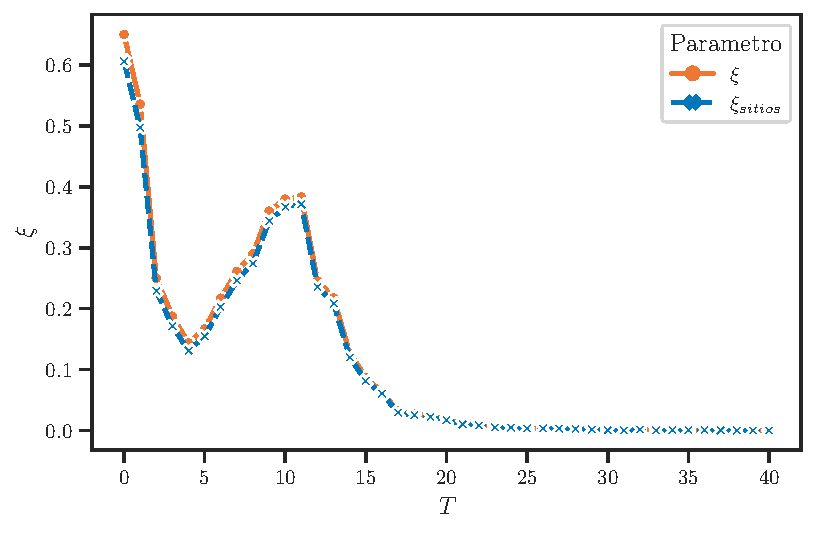
\includegraphics[width=\imsize]{correlacion_modelo.pdf}
	\caption[ Grafico de $\xi$ en función de $T$ para nuestro modelo.  ]{ Grafico de $\xi$ en función de $T$ para nuestro modelo. Observamos que $\xi$ diverge cuando $T \to T_c$ . Observamos que la longitud de correlación no diverge, sino que tiene un pico  como resultado del tamaño finito del sistema. } \label{fig:correlacion_modelo}
\end{figure}










%\section{Discusión}
%
%
%La cuantificación de la evolución espaciotemporal del grupo demuestra avalanchas sin escala que se propagan en estructuras de tipo fractal (con una dimensión ligeramente mayor que dos, véase la Fig. 2F, la Fig. 2G y la Fig. 2H). Este resultado es una confirmación de lo que se conocía previamente para la dinámica cerebral a escalas más pequeñas mediante experimentos electrofisiológicos [12]. Sin embargo, destaca el hecho de que las predicciones basadas en las propiedades del estado crítico se manifiestan en todas las escalas espaciales y temporales de la dinámica cerebral. La invariancia de escala dicta que las avalanchas de actividad deben seguir la misma distribución independientemente de su tamaño y que deben encontrarse eventos tan grandes como el tamaño del sistema. 
%
%
%
%Los tres ejemplos son el tipo de grupos (como ya se definió para los resultados de la figura 2) que se encuentran en los regímenes desordenado, intermedio y ordenado. Es solo en el régimen crítico donde se pueden observar grupos de todos los tamaños, que en términos dinámicos representan el equilibrio entre alta integración (pocos grupos grandes) y alta segregación (muchos grupos pequeños). De hecho, esta mezcla se caracteriza por una distribución invariante de escala de tamaños de grupos (ver la figura 2D para la distribución encontrada experimentalmente).**
%
%
%Como reveló la investigación detallada del modelo FHN, la definición de conectividad funcional, a través del coeficiente de correlación cruzada entre las series temporales de dos nodos,  solo es igual en el crtico 
%
%
%
%Para ello, se contrastaron las redes de correlación de la fMRI cerebral humana con las redes de correlación extraídas de simulaciones numéricas del modelo de Ising en 2D, a diferentes temperaturas. Para la temperatura crítica Tc, aparecen similitudes sorprendentes (como se muestra en la Figura 3.2) en las propiedades estadísticas más relevantes, lo que hace que las dos redes sean indistinguibles entre sí. Estos resultados se interpretaron como un apoyo adicional a la conjetura de que la dinámica del cerebro en funcionamiento está cerca de un punto crítico.
%
%
% Esta distribución también se encontró en el modelo de Ising y Kuramoto [51] en el estado crítico, lo que sugiere que los datos exhibían criticidad. 
% 
% 
% Se obtuvieron diferentes dinámicas cambiando la excitabilidad de los nodos, pero solo los resultados recopilados en criticidad se compararon bien con la fMRI humana. Estos sorprendentes resultados indican que la actividad cerebral espaciotemporal en la RSN humana representa un fenómeno emergente colectivo exhibido por la estructura subyacente solo en criticidad. Al indicar bajo qué condiciones dinámicas específicas la estructura del cerebro producirá la conectividad funcional observada empíricamente, los resultados de Haimovici no solo enfatizaron que "la misma red estructural puede soportar una amplia gama de estados dinámicos y cognitivos", sino que también mostraron, por primera vez, cómo se puede hac
% 
% Motivado por nuestras observaciones de ondas espirales fisiológicas, uno de nosotros desarrolló un nuevo análisis estadístico adecuado para caracterizar cuantitativamente dichas ondas (Jung, 1997). El análisis produce distribuciones de tamaño, p(s)  s0a , que, tanto para datos numéricos como biológicos, se describen con precisión mediante leyes de potencias con exponentes a bastante similares. En el SNC sano, la señalización de largo alcance por iones de calcio probablemente ocurre a través de estas ondas coherentes.
% 
% 
% En primer lugar, hemos introducido un nuevo modelo de red probabilístico que puede capturar la dinámica de propagación espacio-temporal de las convulsiones en redes cerebrales complejas específicas del paciente. 
% 
% 
% Esta es la primera demostración de que un enfoque de modelización híbrido (conectividad anatómica realista más una regla dinámica simple) es suficiente para capturar aspectos espaciotemporales relevantes de la dinámica cerebral, siempre que el régimen dinámico sea crítico. Estos aspectos incluyen características genéricas de los sistemas críticos, pero también la emergencia de estructuras que tienen un significado neurobiológico bien establecido, a saber, la RSN cortical. Si bien la evidencia experimental de las firmas de criticidad mencionadas anteriormente en los sistemas cerebrales ya había sido discutida [8], aquí hicimos un punto más fuerte: en el modelo, el régimen crítico aparece como una condición necesaria para la emergencia de aspectos neurobiológicamente relevantes de la dinámica cerebral.
% 
% Las redes de estado de reposo simuladas exhibieron patrones espaciales más realistas en presencia de principios de plasticidad homeostática
% 
% 
% 
% discusion final 
% 
% El modelo que presentamos es un "modelo de juguete" que simplifica brutalmente los verdaderos procesos neurofisiológicos subyacentes. Precisamente por su sencillez, los modelos de juguete son útiles como primeras aproximaciones al análisis de sistemas complejos. La indiferencia de las leyes estadísticas a los detalles microscópicos justifica sólo en parte la simplificación despiadada que los modelos deben hacer de la realidad. De hecho, en lugar de insistir en su realismo, estos modelos de juguete se consideran mejor como realidades estilizadas en las que los agentes interactúan en entornos bien definidos, capturando algunos elementos clave de los sistemas reales [43]. En el lenguaje de la mecánica estadística, se podría argumentar que los sistemas críticos están organizados en clases universales [44], donde los detalles microscópicos se vuelven irrelevantes para entender el comportamiento colectivo emergente. Entendemos que la existencia de tales clases universales en los sistemas biológicos es todavía una cuestión controvertida [45, ?], y no presentamos aquí una caracterización exhaustiva de nuestro modelo en términos de exponentes críticos.
% 	Sin embargo, lo que queremos destacar aquí es que este modelo tan simple fue capaz de replicar por primera vez resultados fundamentales de los experimentos de fMRI en estado de reposo, como las redes en estado de reposo. Además, es precisamente su sencillez lo que nos ha permitido hacer hincapié en la relación entre estructura y función: es necesario que haya una dinámica crítica para desvelar las estructuras subyacentes que dan forma a las redes en estado de reposo.
% 	
% 	
% 	Hasta donde sabemos, los resultados presentados en este capítulo constituyen la primera demostración de que un enfoque de modelado híbrido que utiliza conectividad anatómica realista más una regla dinámica simple es suficiente para capturar aspectos espacio-temporales relevantes de la dinámica, siempre que el régimen dinámico sea crítico.
% 	
 	